\chapter{Implementation  and Results}
We have implemented our proposed scheduler and simulated the grid environment with standard worloads. The dispatcher uses Message Passing Interface(MPI) communication environment to interact with the resources and submit jobs. In this chapter implementation methods and experimentation details of scheduler and its performance based on various parameters have been discussed.
\section{Implementation Details}
We have implemented our work in C++ programming language. The job scheduler module schedule jobs. The resource manager simulates the dynamic behaviour of resources in grid. An initial configuration of the online resources is considered before starting the job scheduling process. The dispatcher send jobs to corresponding resources.\\
Implemented system with job scheduler module has following features.
\begin{figure}[t]
    \centering
    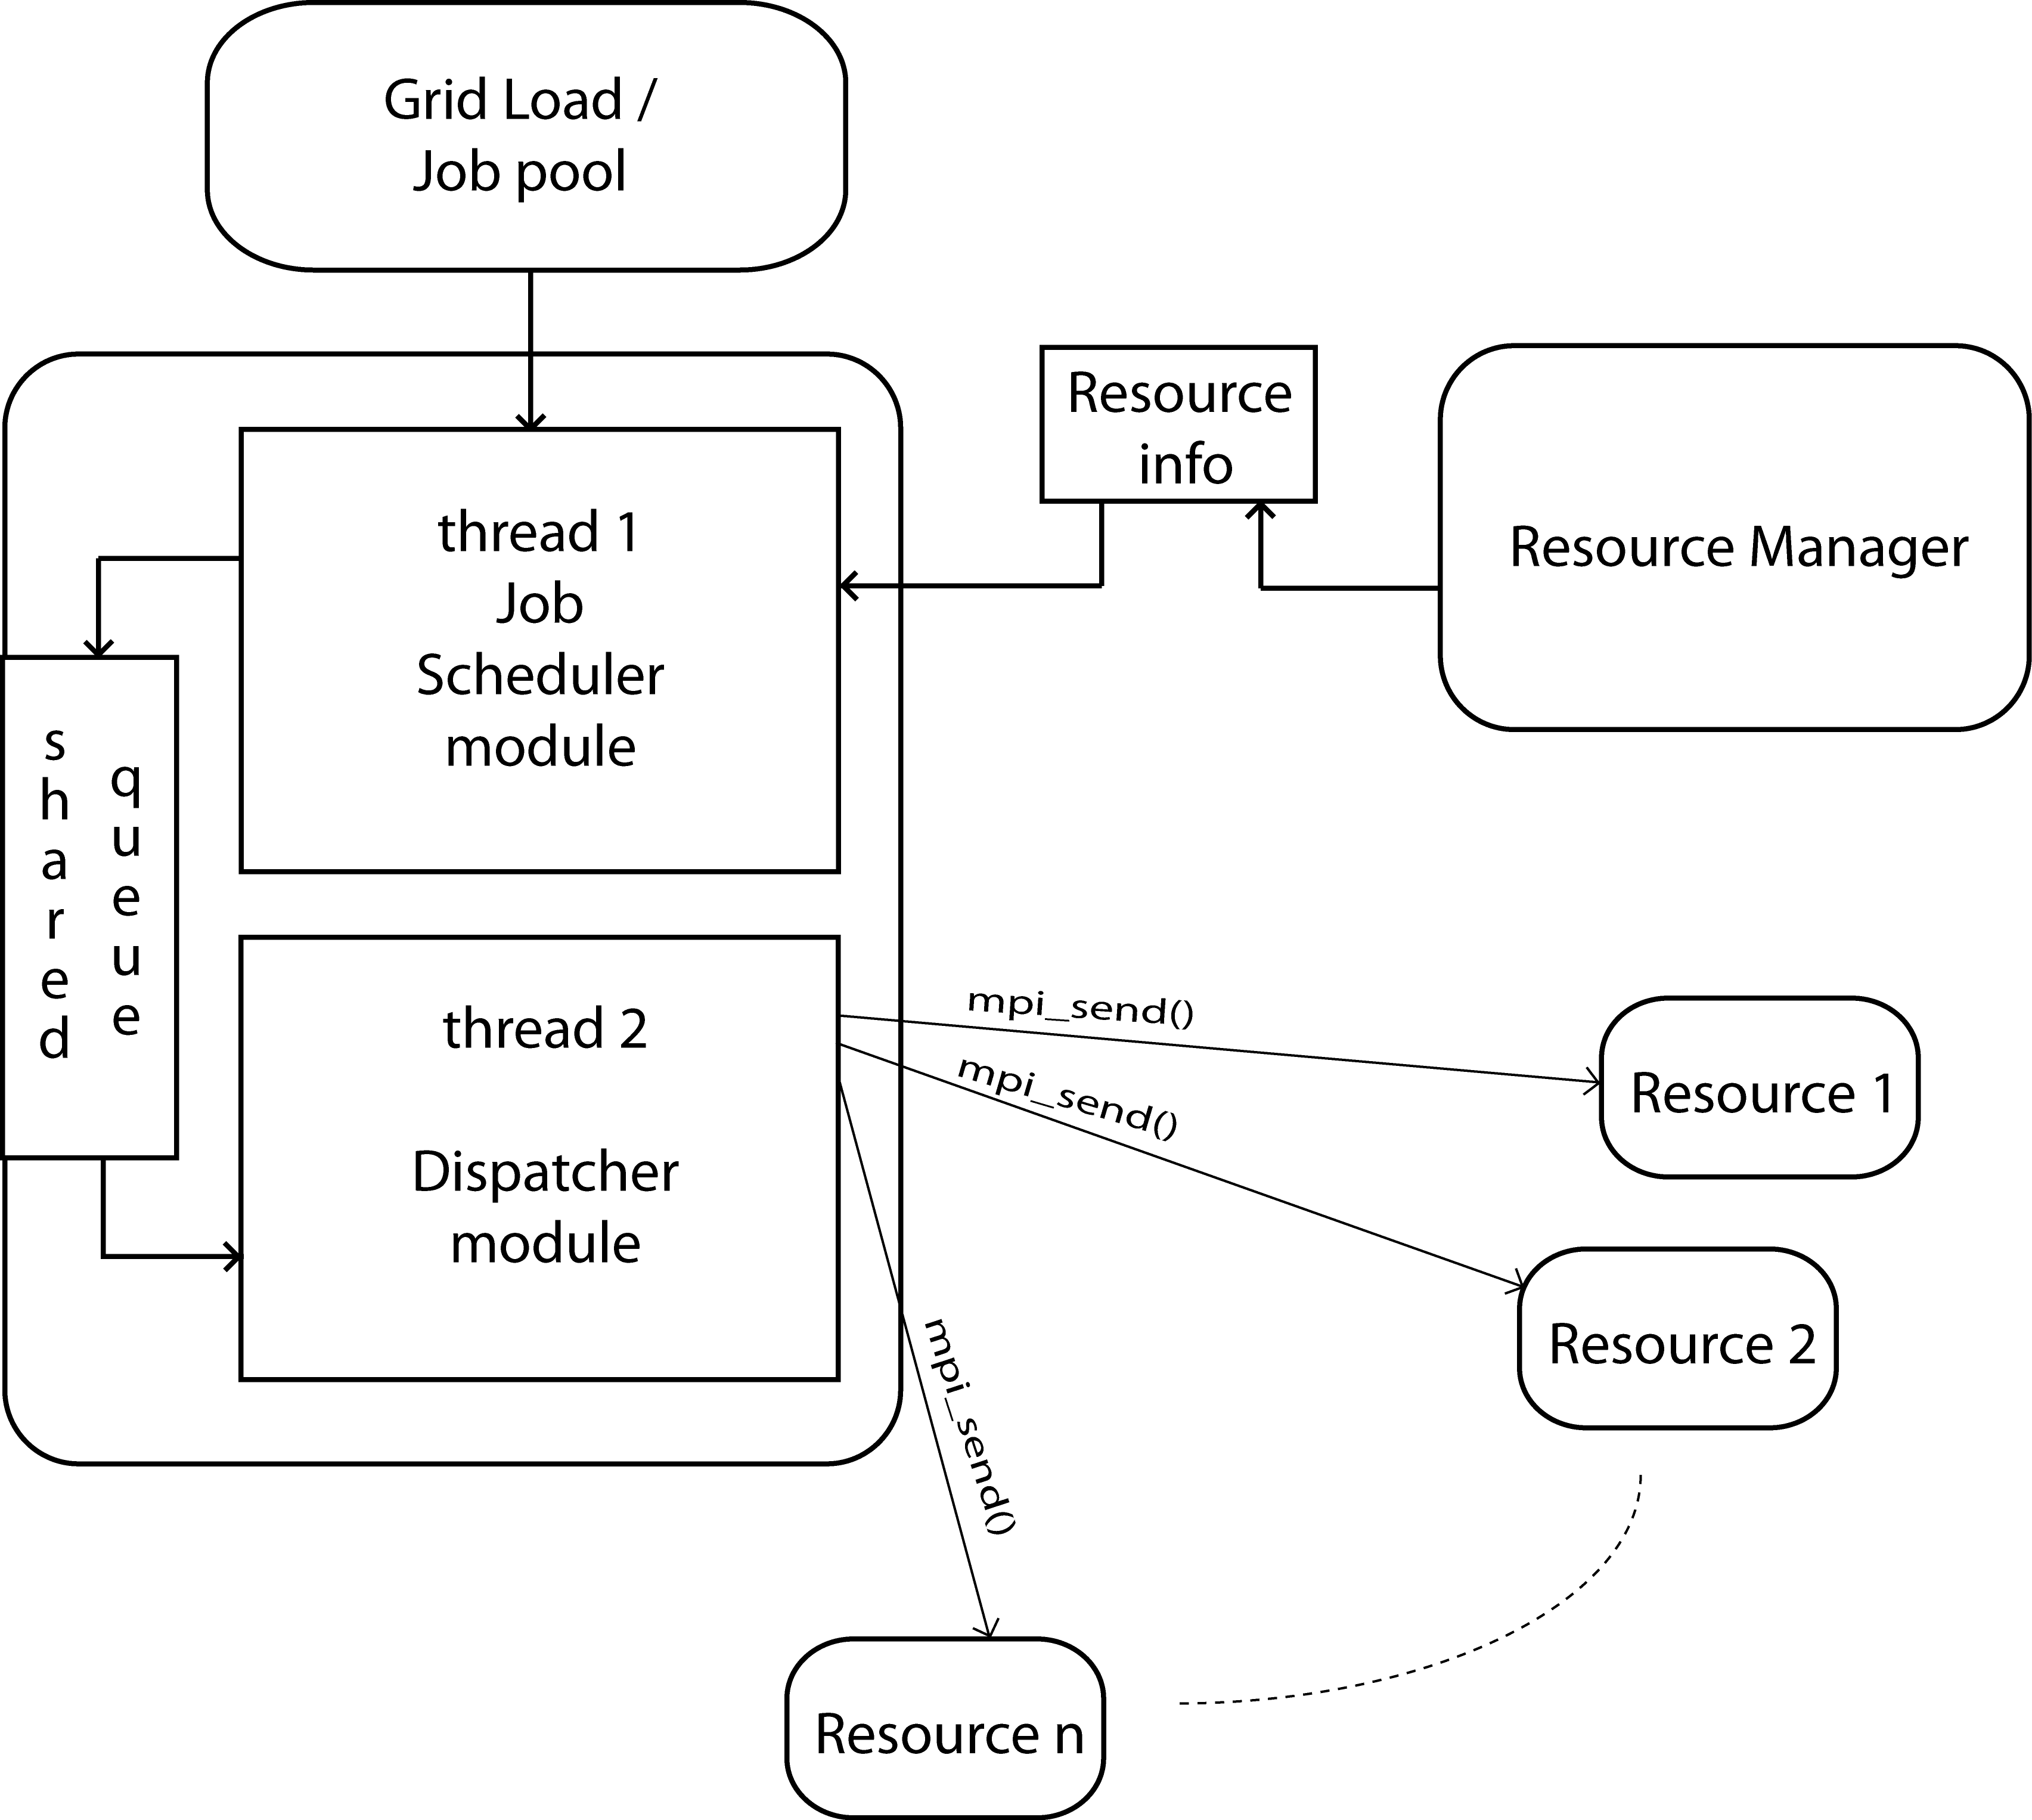
\includegraphics[width=1.0\columnwidth]{implement}
    \caption{Implemented System model}
	\label{fig:Systemmodel}
\end{figure}
\begin{itemize}
 \item Preprocessing of fine-grained jobs for reducing computing complexity of job scheduler.
 \item Flexibility of choosing best scheduling strategy from first pareto front. First pareto front represents non-dominating sets of strategies based on objective parameters.
 \item Normalized weighted sum approach, where weights can be changed dynamically assigned based on the change in grid behaviour.
 \item Configuring resources on the fly. Adding, modifying and deleting resources via resource manager.
 \item Real time job scheduler.
\end{itemize}
\section{System model}
Here we discuss detailed architecture of the implemented system. We have used posix thread to share the scheduling or mapping queues with the dispatcher. The Multi-objective Job Scheduler module run on one thread and dispatcher on another. The scheduler act as a producer and the dispatcher as a consumer. To simulate the grid environment the dispatcher sends job details through MPI to its mapped resource. The resources waiting for the messages on receiving job, run dummy jobs with the parameters passed on to it. Figure~\ref{fig:Systemmodel} is the schematic representation of the implemented system.\\
Dispatcher and scheduler maintains separate queues for separate resources. When  a resource goes down, jobs of that queue is rescheduled on available resources.
\subsection{Job queue}
It have been considered that a job requires a single core of processor for execution. Table~\ref{jobmodel} represents a segment of job queue.
Each grid job has following properties:
\begin{itemize}
 \item $JOB\_ID$ is an unique identifier for a job.
 \item Grid jobs are either CPU intensive or I/O intensive represented as $JOB\_TYPE$ 0/1 respectively.
 \item $PRED\_ID$ is the predecessor job on which the job is dependent. $-1$ represent no dependencies on other job.
 \item $JOB\_SIZE$ of CPU intensive jobs are either represented in MI (Million Instruction). % or Execution time scaled with a fixed MIPS.
 \item $JOB\_SIZE$ of I/O intensive jobs are either represented in MB (Mega Bytes). % or Transfer time scaled with a fixed MBPS.
 \item $TIME\_LIMIT$ is a constraint for job completion, exceeding time limit imposes penalty. Unit of $TIME\_LIMIT$ is seconds.
 \item $JOB\_COST$ is the expected cost to be incurred by the user based on the QoS agreement. Unit of $JOB\_COST$ is currency e.g. USD(\$).
\end{itemize}
\begin{table}[ht]
\caption{User job queue}
    \begin{tabular}{|c|r|c|c|c|c|}
    \hline \hline
    $JOB\_ID$ & $JOB\_SIZE$ & $TIME\_LIMIT$ & $JOB\_COST$ & $PRED\_ID$ & $JOB\_TYPE$ \\ 
     & in MI/MB & in seconds & in \$ &  &  \\ \hline
    $\vdots$ & $\vdots$ & $\vdots$   & $\vdots$ & $\vdots$	     & $\vdots$  \\
    42     & 24,000 MI  & 63.0  & 5.41 & 29                 & 0        \\
    43     & 130,000 MI  & 107.0 & 4.86 & -1                 & 0        \\
    44     & 10,500 MI  & 106.0 & 5.99 & 24                 & 0        \\ 
    47     & 530.0 MB  & 150.0 & 5.04 & 29   	       & 1	\\
    48     & 240,200 MI  & 133.0 & 5.40 & 31   	       & 0        \\
    $\vdots$ & $\vdots$ & $\vdots$   & $\vdots$ & $\vdots$	     & $\vdots$  \\ \hline
    \end{tabular}
\label{jobmodel}
\end{table}
\subsection{Resource model}
Resource manager configures each resource with the following properties. Table~\ref{resconf} shows configuration of some of the resources in grid.
\begin{itemize}
 \item $RESOURCE\_ID$ is an unique identifier for a resource.
 \item Resources are either computing resource or storage resource represented as $RES\_TYPE$ 0/1 respectively.
 \item Computational resource processing capability is measured in MIPS (Million Instruction per second) or IPS(Instruction Per second) per core, and for storage resources it is measured in MB/s. We denote it as $RES\_CAP$ \cite{wiki_CPU}.
 \item Another resource parameter is power dissipation/consumption figure in watts. $RES\_ENERGY$ is also represented in a normalized form \cite{wiki_wattage}.
\end{itemize}
\begin{framed}
{\small
	     Resource power dissipation figure is measured in Watts. Resource with maximum power dissipation figure is found and scaled to 1.0. Similarly other resources power dissipation figures are scaled with maximum power dissipation figure. For example Intel Core i7 920 (Quad core) consumes 130 Watts and Intel Core 2  X6800 (Dual core) consumes 75 Watts, 130 Watts is normalized to 1.0 and 75 Watts to 0.577 \cite{wiki_wattage}.
}
\end{framed}
\begin{itemize}
 \item $RES\_COST$ is the cost of the resource per second.
\end{itemize}
Resources manager module updates available resources information in a file which is being read  by Job scheduler module before each run.
\begin{table}[ht]
\caption{Resource configuration}
    \begin{tabular}{|c|r|c|c|r|}
    \hline \hline
    $RESOURCE\_ID$ & $RES\_COST$ & $RES\_TYPE$ & $RES\_ENERGY$  & $RES\_CAP$ \\ 
     & in \$ &  & \emph{normalized}  & {\small in MIPS/MBPS} \\ \hline \hline
    $\vdots$ & $\vdots$ & $\vdots$   & $\vdots$ & $\vdots$  \\
    4 & 0.13 & 0 & 0.943 & 9,726 MIPS   \\
    5 & 0.14 & 0 & 1.000 & 29,621 MIPS   \\
    6 & 0.13 & 0 & 0.577 & 13,539 MIPS \\
    7 & 0.11 & 1 & 0.894 & 30.0 MBPS     \\
    $\vdots$ & $\vdots$ & $\vdots$   & $\vdots$ & $\vdots$  \\ \hline
    \end{tabular}
\label{resconf}
\end{table}

\subsection{Output of scheduler}
The scheduler yields mapping of jobs and resources with start time and expected execution time of each job. Each resource has its own queue. A queue of jobs mapped to resource id 1 is shown in Table~\ref{tab:out}
\begin{table}[ht]
\caption{Mapping queue for RESOURCE\_ID 1}
 \centering
    \begin{tabular}{|c|c|r|r|}
    \hline \hline
    $JOB\_ID$ & $RES\_ID$ & $START\_TIME$ & $EXEC\_TIME$ \\ 
     &  & in seconds & in seconds \\ \hline \hline
    $\vdots$ & $\vdots$ & $\vdots$   & $\vdots$ \\ 
    95255	& 1	& 952.42	& 138.30 \\ 	
    95259	& 1	& 1090.73	& 78.58 \\ 
    95205	& 1	& 1169.31	& 37.71 \\ 
    95306	& 1	& 1207.03	& 62.86 \\ 
    95301	& 1	& 1269.90	& 59.72 \\ 
    95337	& 1	& 1329.62	& 194.88 \\
    $\vdots$ & $\vdots$ & $\vdots$   & $\vdots$ \\ \hline \hline
    \end{tabular}
\label{tab:out}
\end{table}

\subsection{Randomize function}
In any stochastic algorithm randomize function plays an important role. A very fast random number generator Mersenne Twister of period $2^{19937}-1$ is used in different parts of the code and has a better equidistibution property. It generates integer in the range $0$ to $2^{32}-1$ and real number range $[0,1)$ with a precision of $2^{32}$ \cite{saito2007application}.

\section{Data Sets}
\label{datasets}
Standard grid workload from Grid Workload Archive have been used in this experiments \cite{gridload}. The traces and logs of different grid environments are given in standard gwf format. Gridloads are processed to add a few more parameters like cost of jobs, jobs time limit for completion, predecessor dependencies among jobs and type of jobs. \\
SHARCNET \& DAS-2 are the two traces that have been processed. Traces shows that execution time of jobs ranges from 1 to 20000 time units in DAS-2, and 1 to 100000 time units in SHARCNET. This shows job characteristic varies widely making scheduler task difficult.\\
For analyzing the performance based on various parameters following workloads have been created given in Table ~\ref{tab:gridlet}.

\begin{table}[ht]
\caption{Gridlet configuration}
\centering
    \begin{tabular}{|c|c|c|c|}
    \hline \hline
    Workload\_id & Trace        & Precedence constraint & Resource constraint \\ \hline
    1 	         & DAS-2    & \xmark                 & \xmark   \\
    2 	         & SHARCNET & \xmark                 & \xmark   \\
    3 	         & DAS-2    & \xmark                 & \cmark   \\
    4 	         & SHARCNET & \xmark                 & \cmark   \\
    5	         & DAS-2    & \cmark                 & \xmark   \\
    6	         & SHARCNET & \cmark                 & \xmark   \\
    7	         & DAS-2    & \cmark                 & \cmark   \\
    8 	         & SHARCNET & \cmark                 & \cmark   \\ \hline \hline
    \end{tabular}
\label{tab:gridlet}
\end{table}
\begin{framed}
 Workloads are created on the basis of imposing constraints on traces. Job precedence rule is referred to as precedence constraint and constraint of executing jobs on particular type of resource is referred to as resource constraint. Predecessor jobs have been created with the statistics given in table~\ref{pcons}
\end{framed}
\begin{table}[h]
\caption{Precedence Constraints}
\centering
    \begin{tabular}{|c|c|}
    \hline \hline
    Percentage of Jobs & 50\%  \\ \hline \hline
    Range & [JOB\_ID -100 , JOB\_ID -1] \\ \hline
    Mean  & [JOB\_ID -50] \\ \hline
    Variance & 20 \\ \hline \hline
    \end{tabular}
\label{pcons}
\end{table}

\section{Results}
In order to evaluate the performance of our scheduler we have performed set of experiments on the workloads mentioned in section~\ref{datasets}. The scheduler can schedule 200 jobs in 21 seconds. For more optimized results chromosome population and iteration in our algorithm can be increased. 
\subsection{Experiment on independent jobs}
Experiment results given in Figure ~\ref{fig:10res},~\ref{fig:15res},~\ref{fig:20res},~\ref{fig:25res} on workload 1 and 2 shows minimization of makespan and proper utilization of resources on independent jobs. 
Result shows that irrespective of the large variation of granularity in grid jobs we have achieved 99\%+ utilization performance in almost every resource. Result shows the scalability of our scheduler, we have tested the scheduler with 5000, 10000, 15000, 20000, 25000 jobs; and on 10, 15, 20, 25 resources. This shows that scheduler can process large amount of gridlets and resources without compensating on the Makespan and utilization of resources. The scheduler have yield near optimal mapping strategy optimizing on the time limit limit penalty and cost penalty referred in section ~\ref{formulation}.
\begin{figure}[!ht]
    \centering
    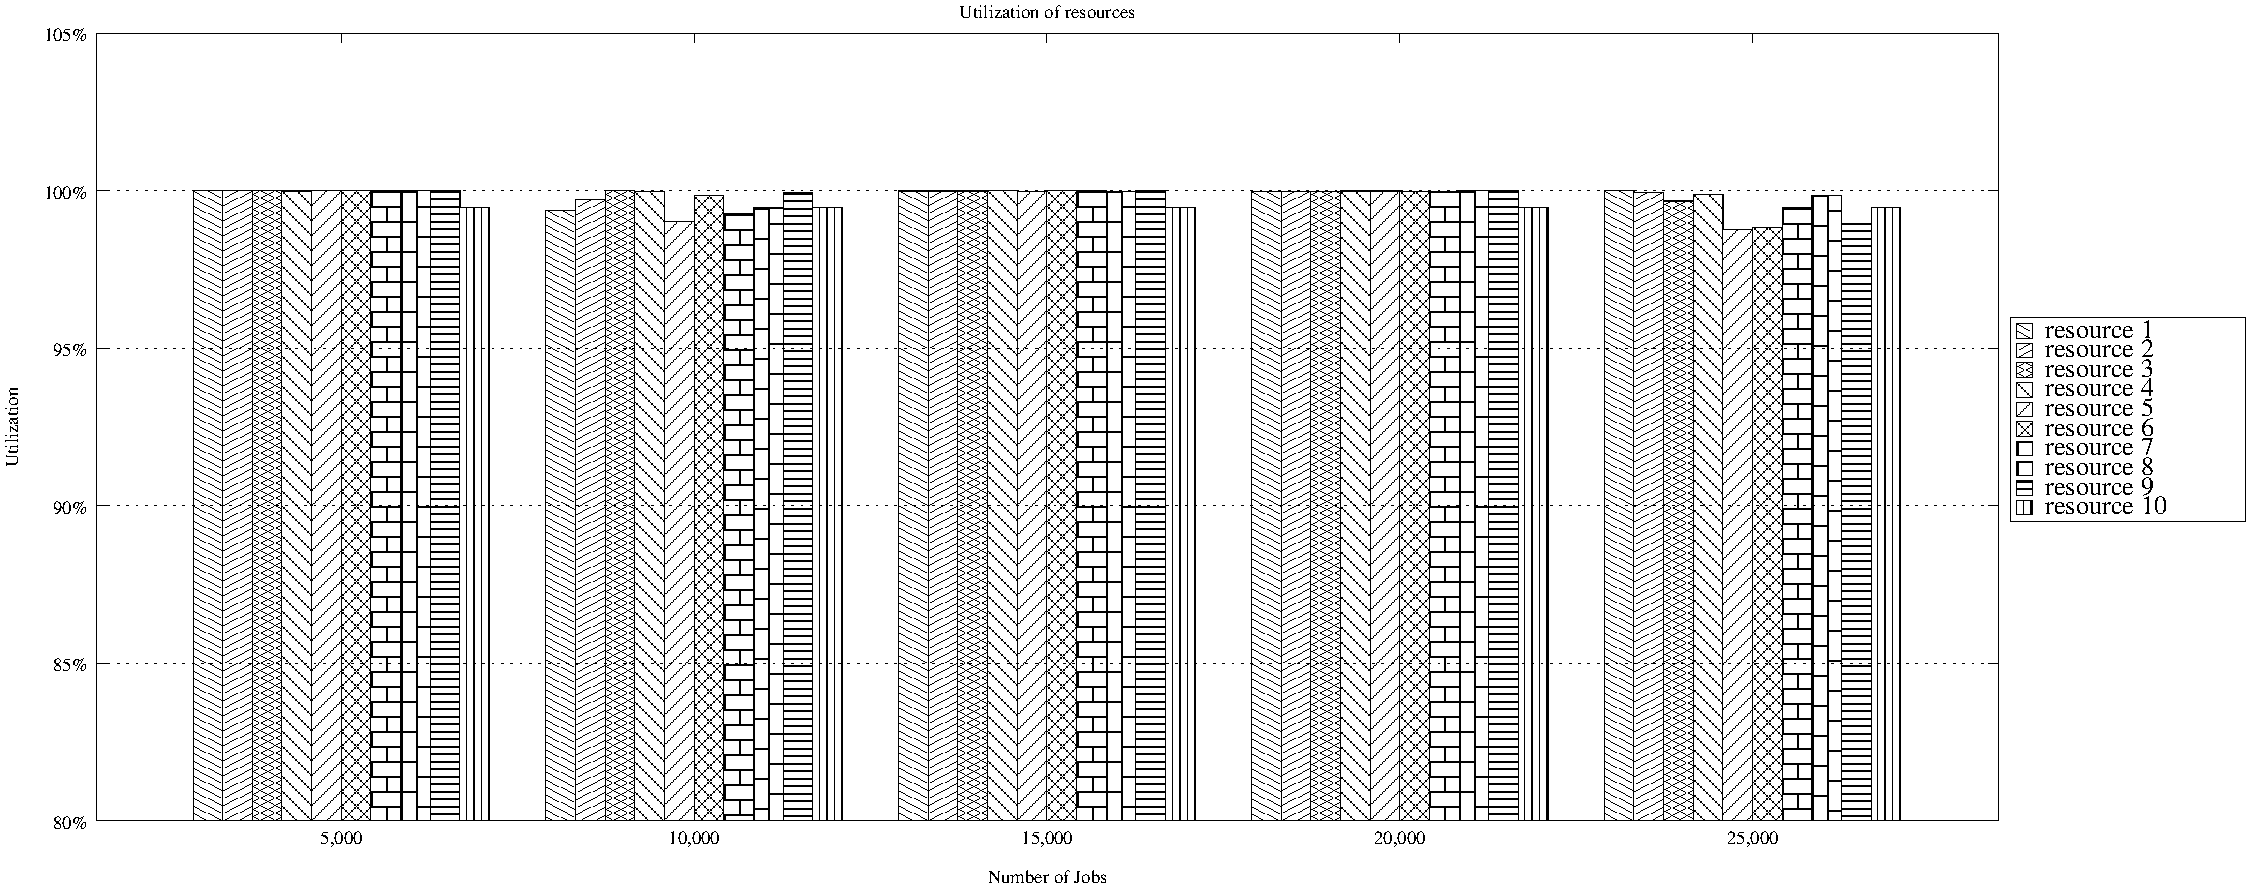
\includegraphics[width=1.5\textwidth,keepaspectratio,angle=90]{10res_SHARCNET}
    \caption{Evaluation of makespan and utilization on 10 resources on workload 2}
    \label{fig:10res}
\end{figure}
\begin{figure}[!ht]
    \centering
%    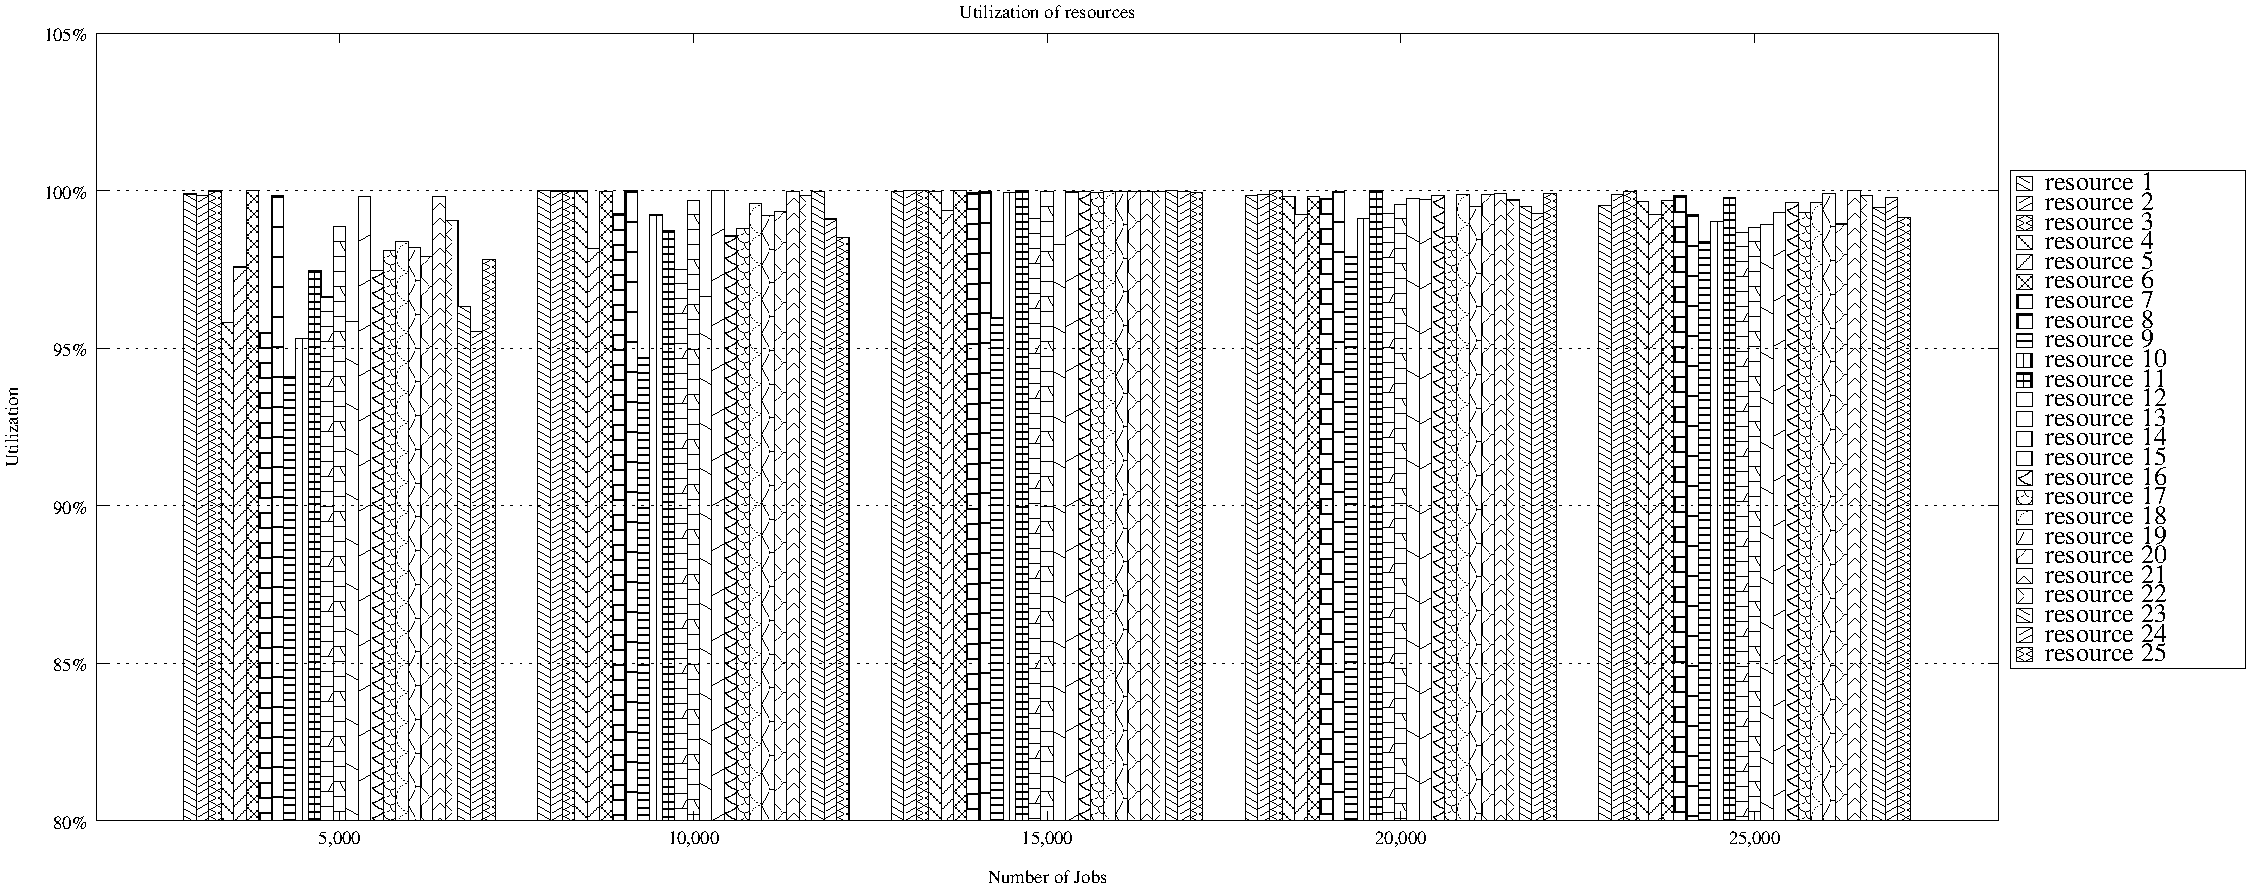
\includegraphics[width=1.1\columnwidth]{25res_SHARCNET}
%    \subfigure[\small ]{
    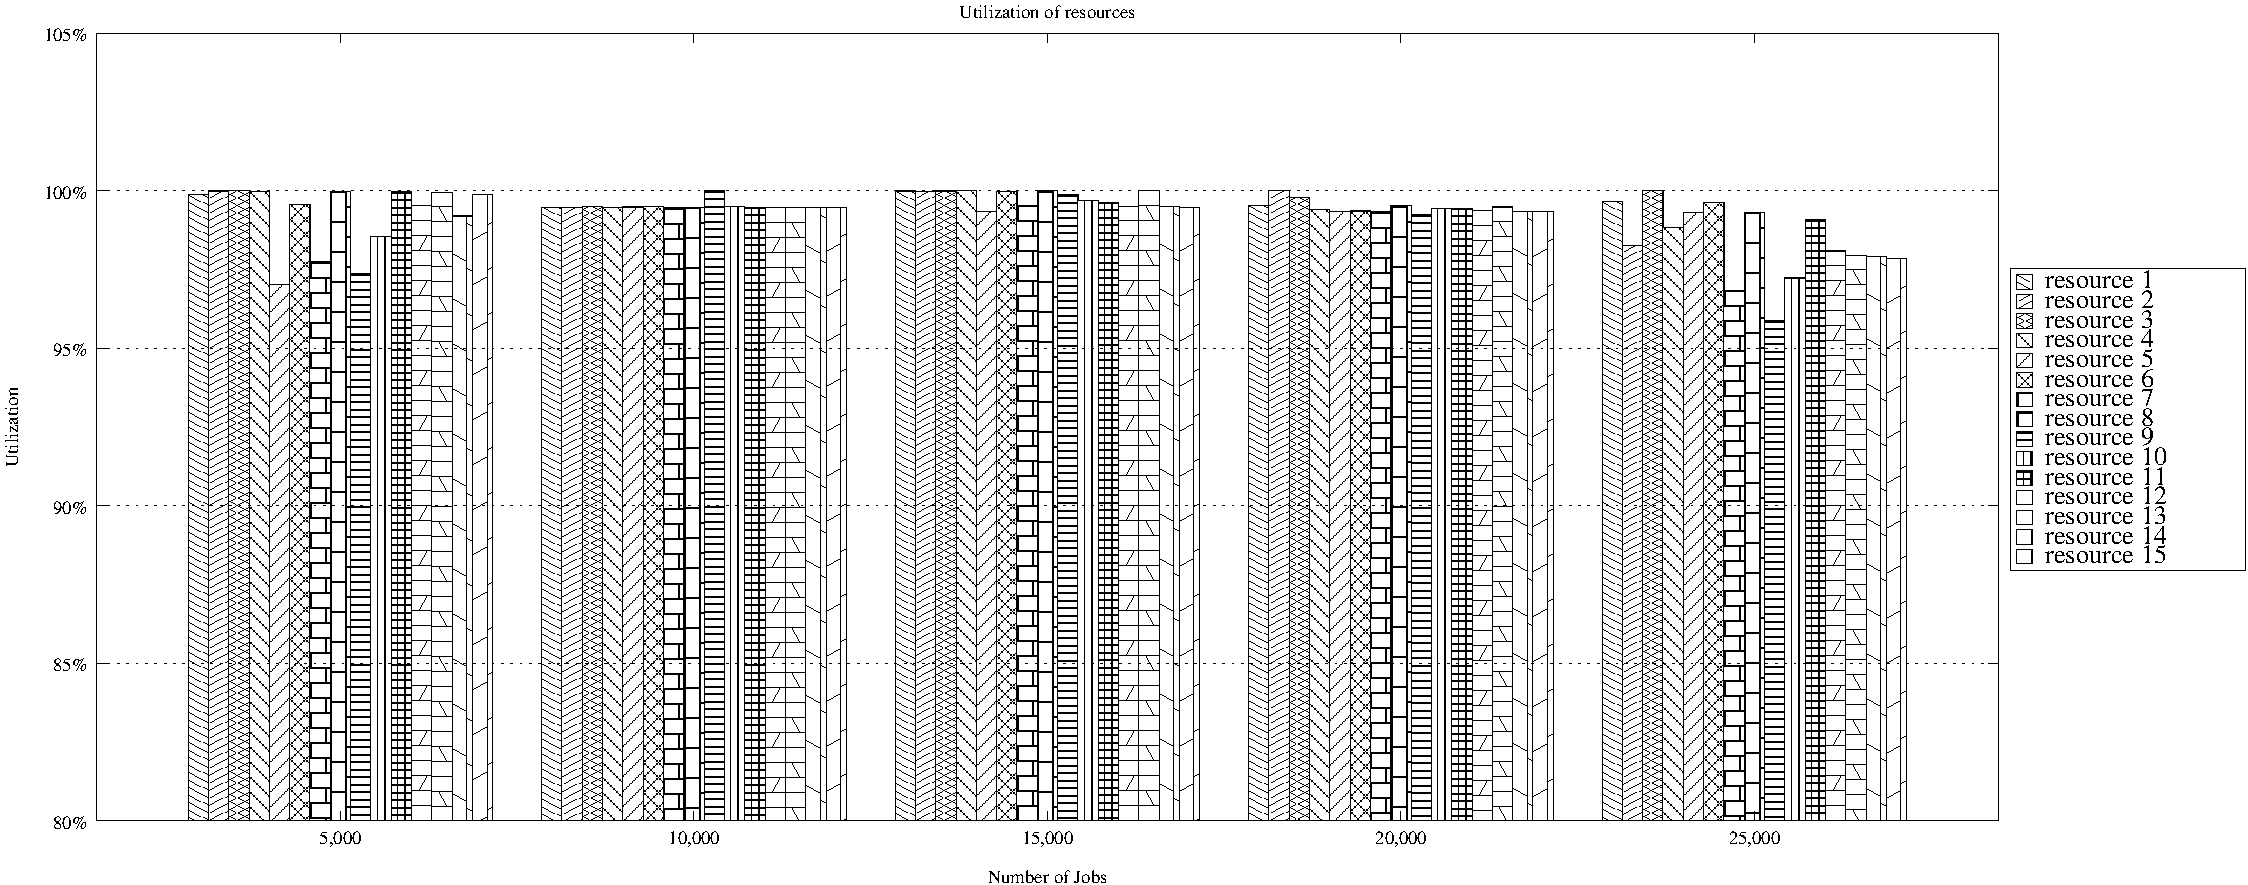
\includegraphics[width=1.5\textwidth,keepaspectratio,angle=90]{15res_SHARCNET}
    \caption{Evaluation of makespan and utilization on 15 resources on workload 1}
    \label{fig:15res}
\end{figure}
\begin{figure}[!ht]
    \centering
    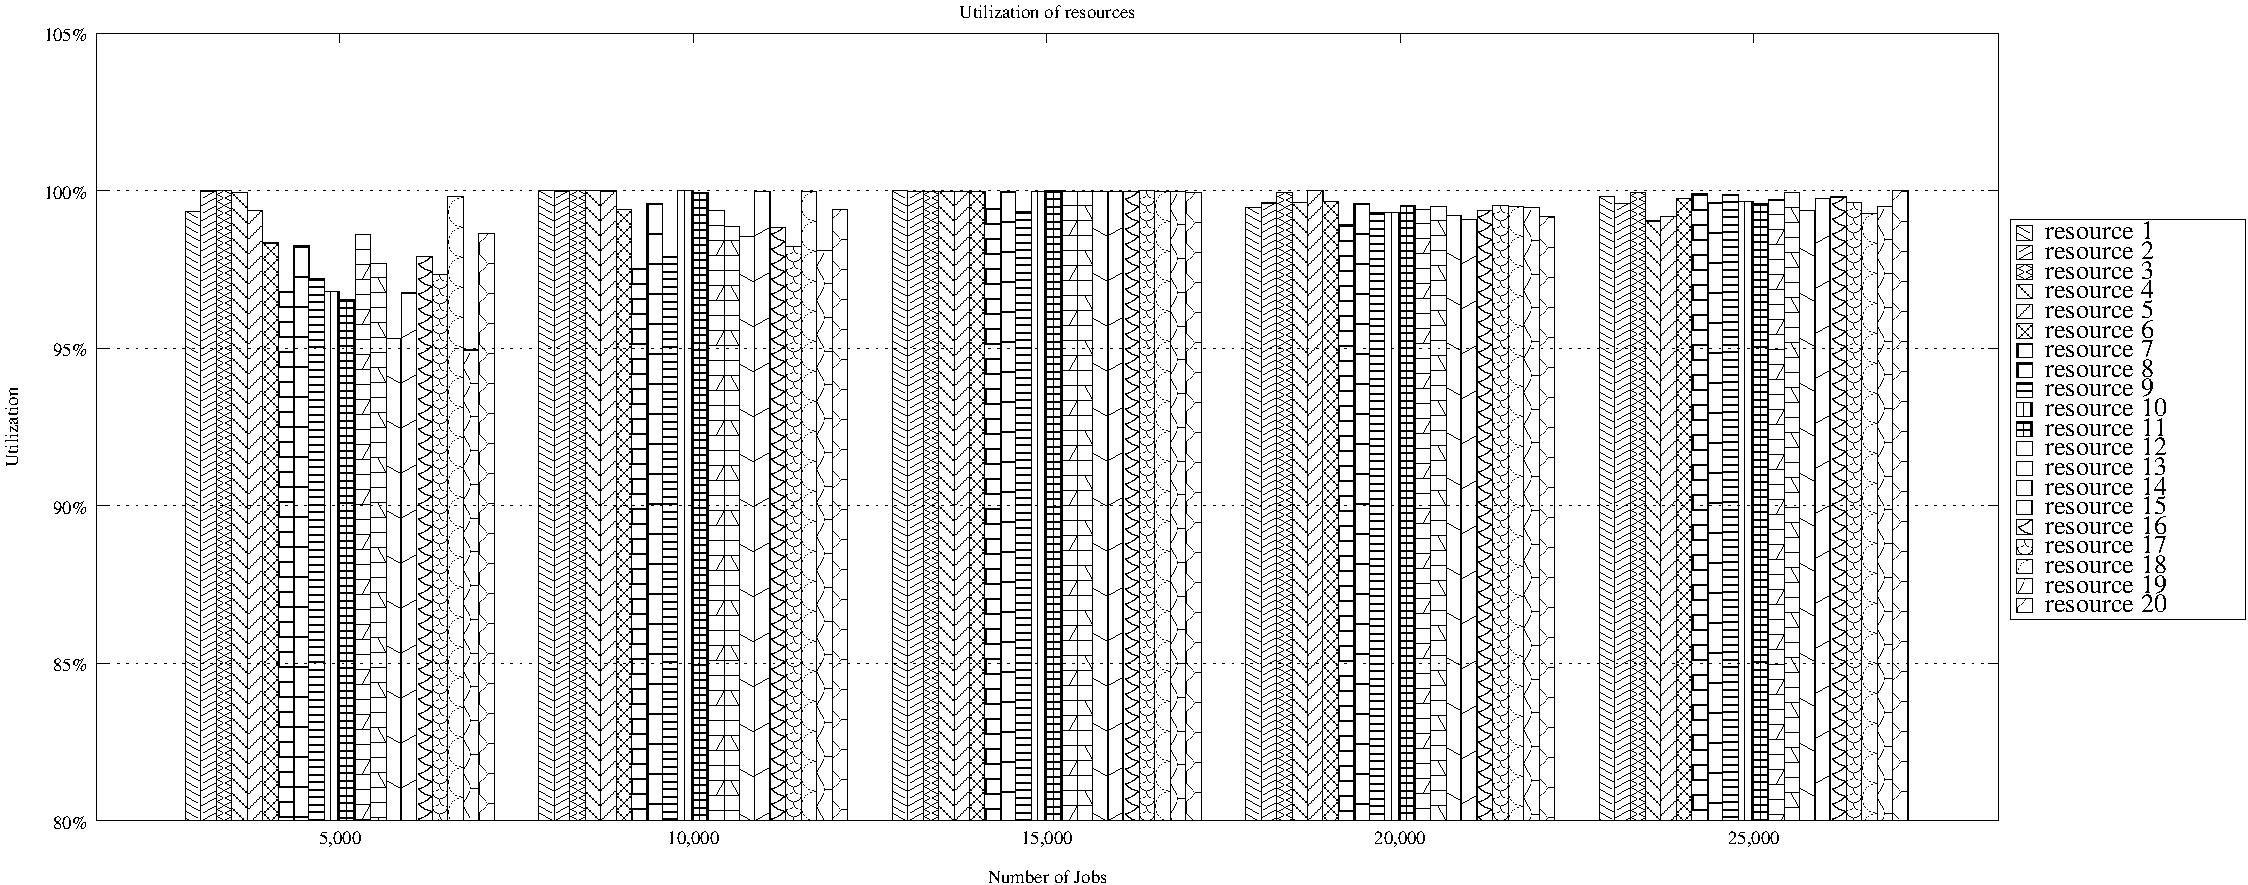
\includegraphics[width=1.5\textwidth,keepaspectratio,angle=90]{20res_SHARCNET}
    \caption{Evaluation of makespan and utilization on 20 resources on workload 1}
    \label{fig:20res}
\end{figure}
\begin{figure}[!ht]
     \centering
    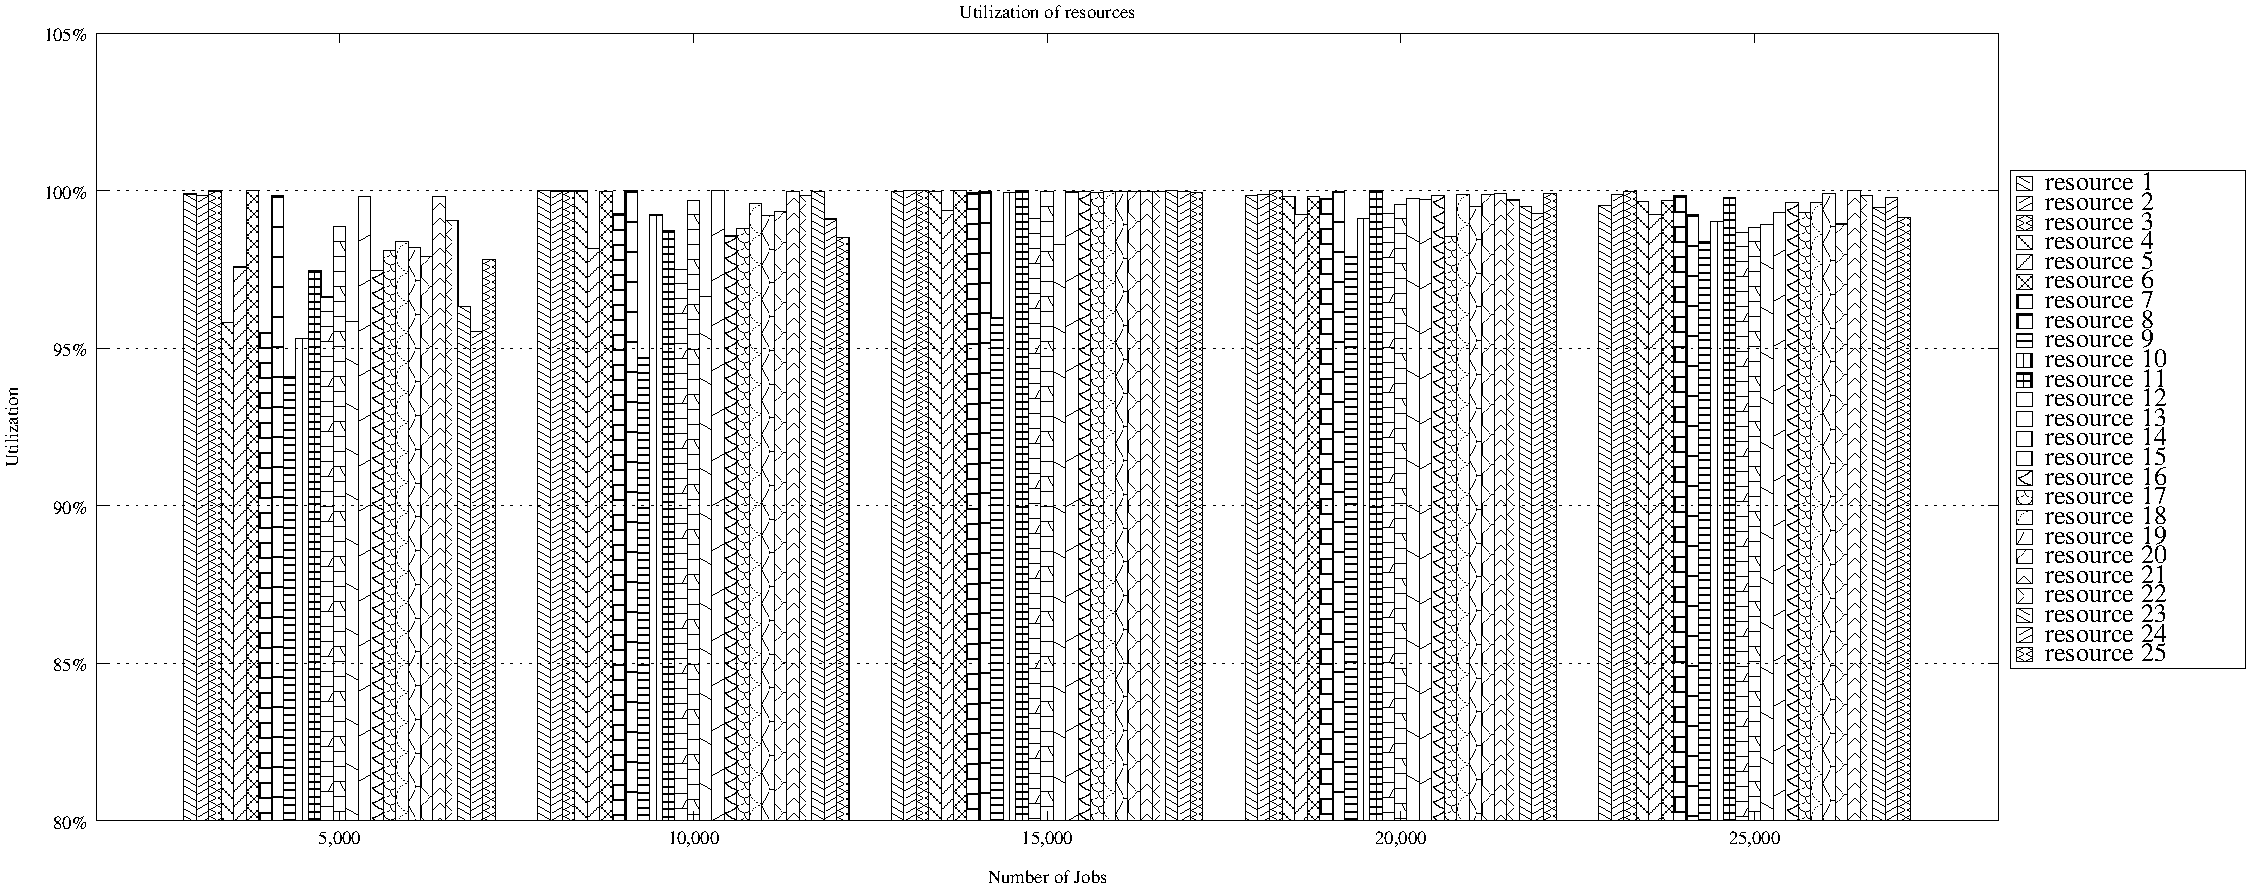
\includegraphics[width=1.5\textwidth,keepaspectratio,angle=90]{25res_SHARCNET}
    \caption{Evaluation of makespan and utilization on 25 resources on workload 2}
    \label{fig:25res}
\end{figure}
\subsection{Trade off between energy consumption and performance}
\label{case2}
\begin{figure}[h]
\centering
  \subfigure[\small Workload 2 (SHARCNET)]{
    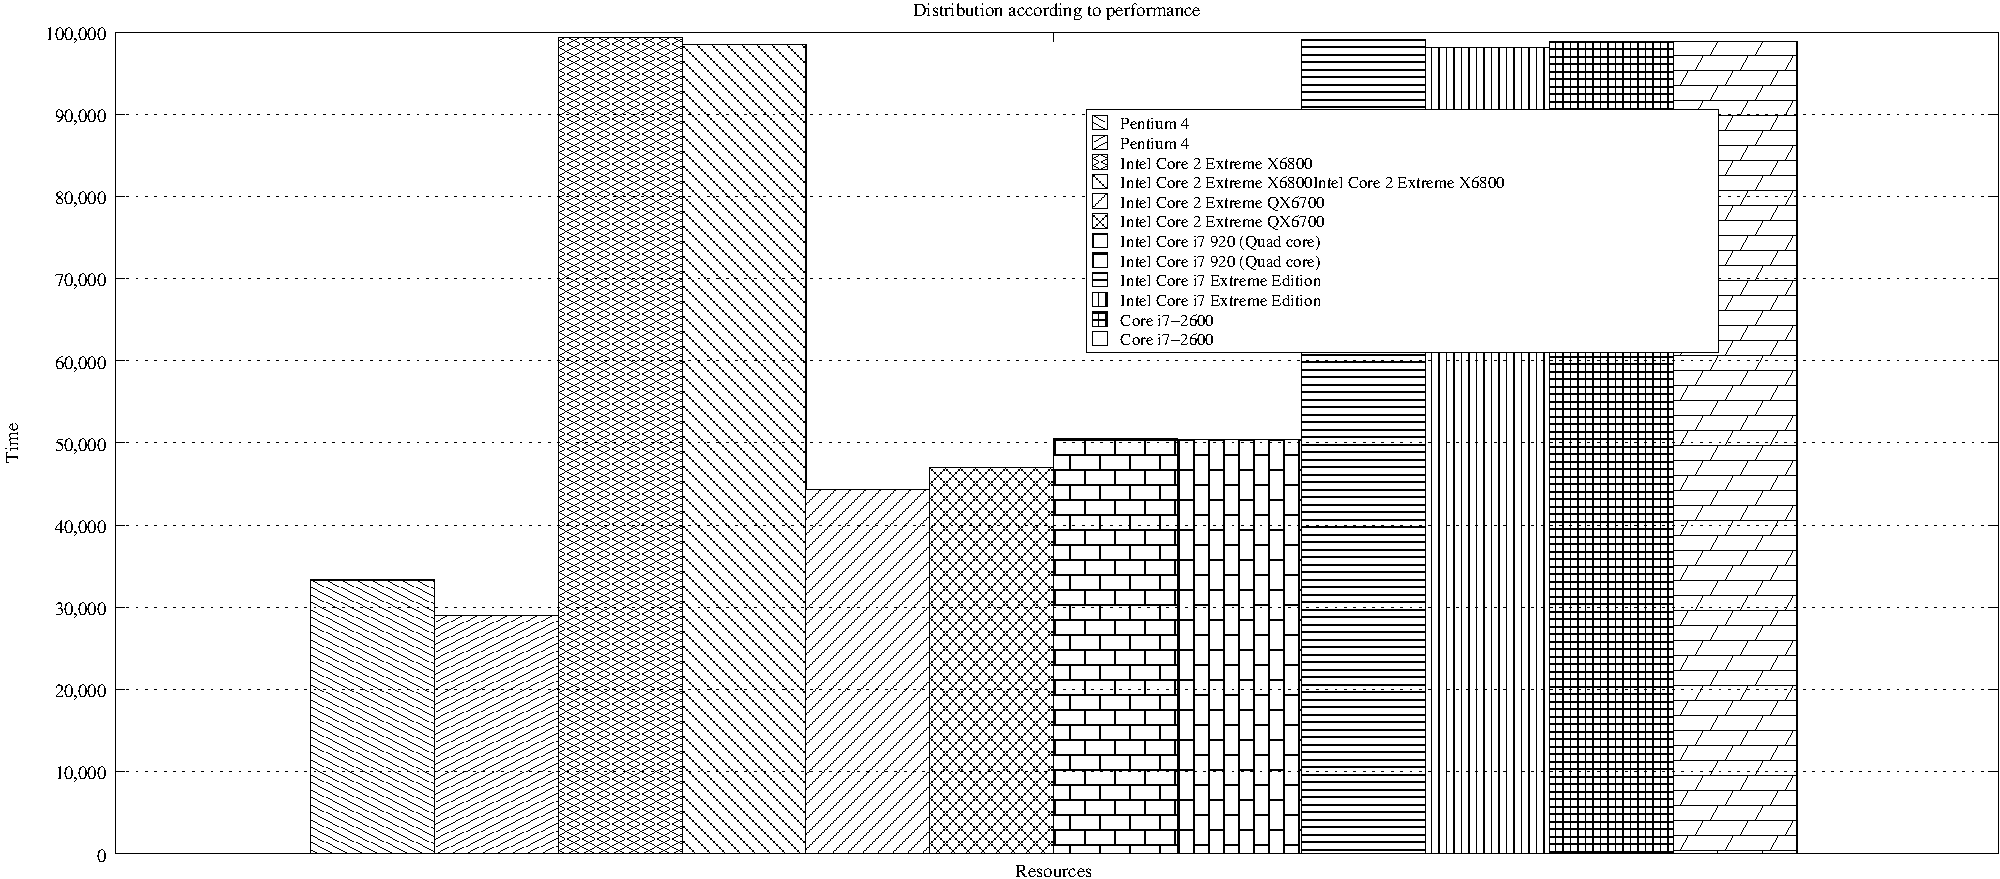
\includegraphics[width=1.0\columnwidth]{case2SHARCNET}
    \label{perform}
    }
    \subfigure[\small Workload 1 (DAS-2)]{
    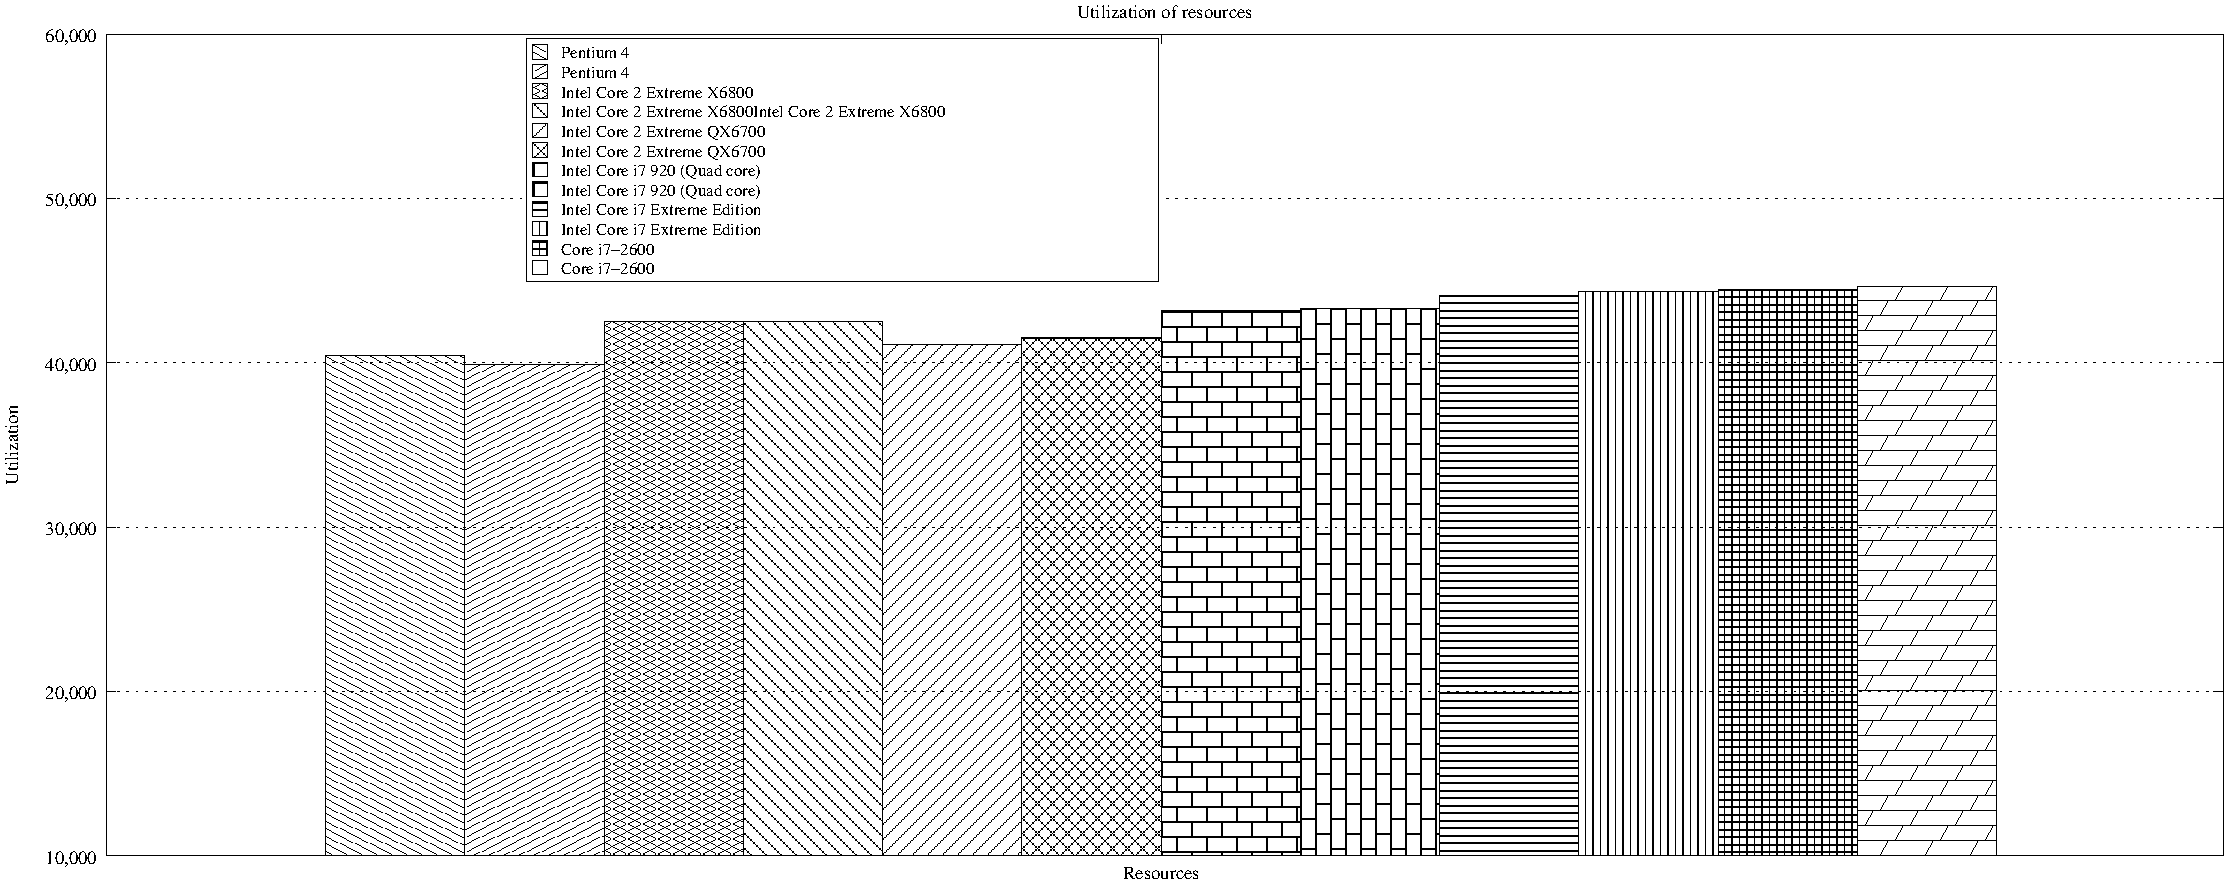
\includegraphics[width=1.0\columnwidth]{case2DAS}
    \label{perform1}
    }
\caption{ Evaluation of Ultilization on workload 1  and 2}
\end{figure}
Now energy parameter and performance parameter is considered while scheduling. It is worthy to note that if job is scheduled on high performance resource less time will be required for job completion and time limit constraint can be satisfied. Again, a job will try to be mapped on a  energy efficient resource minimizing overall power consumption. \\
Usually resources with high performing capability are less energy efficient. Jobs having large time limit can afford to be scheduled on low performance resource with low power consumption figures without being penalized for exceeding time limit. However high priority jobs needs high performance resource to process jobs within time limit.\\
The results given in Figure~\ref{perform} have been obtained by assigning equal weights on performance and energy efficiency objective on pareto front~\ref{pareto}.
Resource configuration for this experiment is given in Table~\ref{tab:res}.
\begin{table}[ht]
\caption{Resource configuration for experiment on workload 1 and 2 }
\centering
    \begin{tabular}{|l|l|c|c|c|}
    \hline \hline
    Machine & Frequency & Watts & MIPS/core & Resource\_id \\ \hline
Pentium 4 Extreme Edition 	&	3.2 GHz 	&	92.1	& 	9,726	 & 1,2 \\ \hline
Intel Core 2  X6800 (Dual core) 	&	2.93 GHz	&	75	&	13,539	& 3,4 \\ \hline
Intel Core 2  QX6700 (Quad core) 	&	2.66 GHz 	&	95	&	12,290 & 5,6	 \\ \hline
Intel Core i7 920 (Quad core) 	&	2.667 GHz 	&	130	&	20,575	 & 7,8 \\ \hline
Intel Core i7 3960X (Hex core) 	&	3.3 GHz	&	130	&	29,621	& 9,10  \\ \hline
Core i7-2600 	&	3.4 GHz	&	95	&	32,075	 & 11, 12 \\ \hline
\end{tabular}
\label{tab:res}
\end{table}
Experiment result for workload 2 is shown in Figure~\ref{perform}. Pentium 4 being poor in performance and energy dissipation factor as compared to other resources, have less uptime or running time. Now comparing resources Core 2 X6800 with Core 2 QX6700, they have almost same MIPS specification but Core 2 X6800 consumes less power. Figure~\ref{perform} shows that scheduler have allocated more jobs in Core 2 X6800 which is reasonable. Same logic can be applied for resources Core i7 920 and Core i73960X. They have same energy dissipation factor but Core i7 3960X performance is better. As a consequence scheduler have scheduled more jobs on Core i7 3960X. Best resource of the lot is Core i7-2600. The scheduler have uniformly distributed jobs among Core 2 X6800, Core i7 3960X and Core i7-2600 to have a minimum makespan.\\
Since workload 2 has large variation in the granularity of jobs the graph shows a worst case analysis in their utilization. In the best case scheduler will try to schedule jobs such that running time on each resource is same ~\ref{perform1}. \\
Figure~\ref{pareto} shows how our scheduler gives a better grip to the administrator to trade off between user objectives and grid administrator objectives. Each point on the space represents a scheduling strategy. In a 3D co-ordinate system we represents 3 objectives which are needed to be minimized namely (i) makespan (ii) Energy efficiency parameter, (iii) time targidity. Any point in the first pareto front can be chosen for scheduling strategy. This gives grid administrator wide range of choices and cope up with dynamic behaviour of grid.

\begin{figure}[h]
\centering
    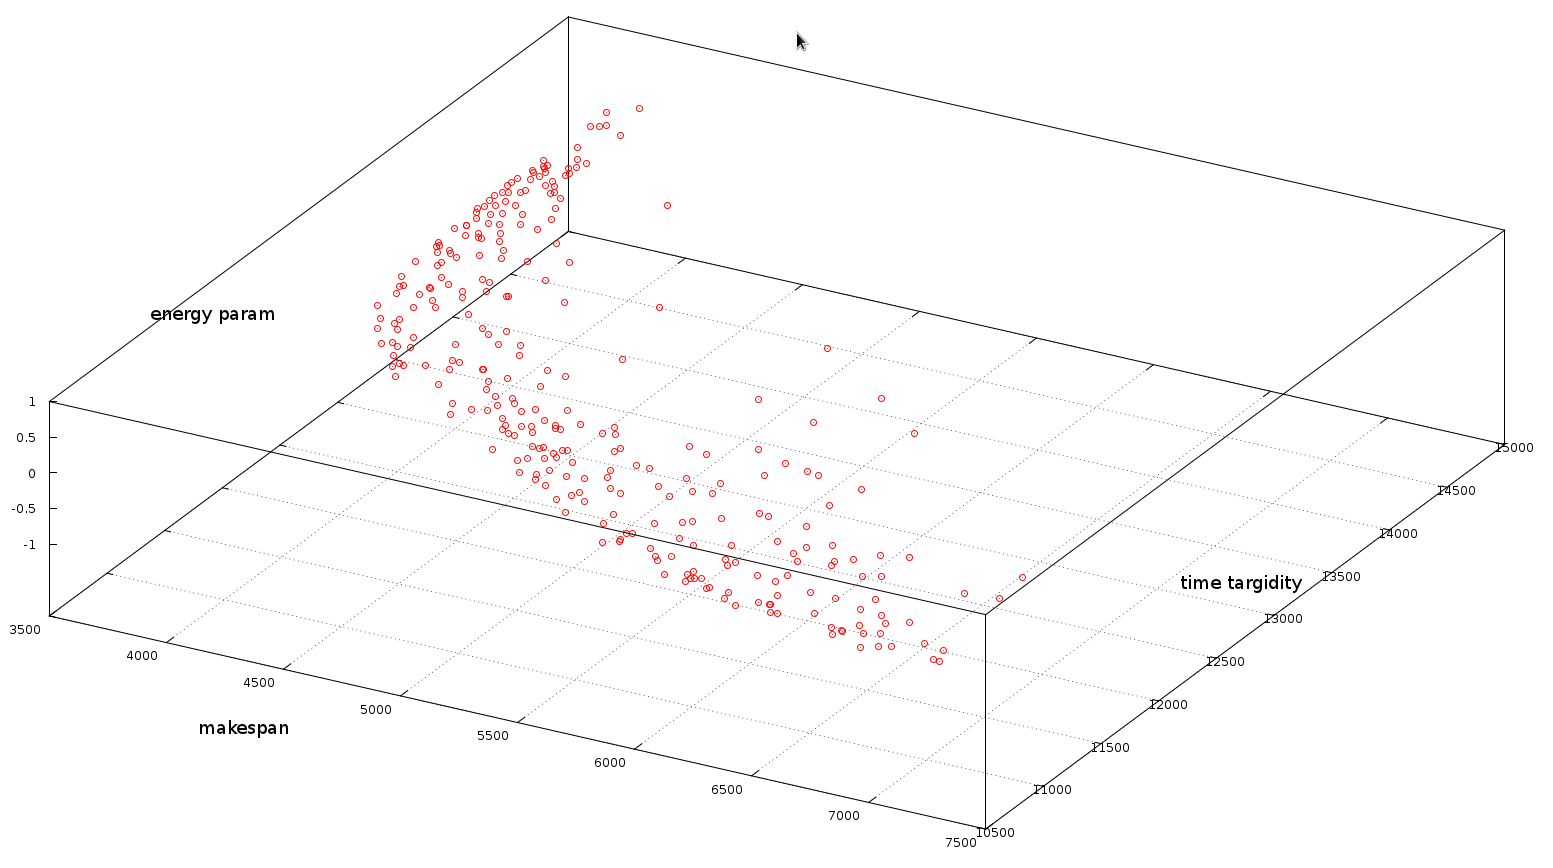
\includegraphics[width=1.0\columnwidth]{pareto2}
    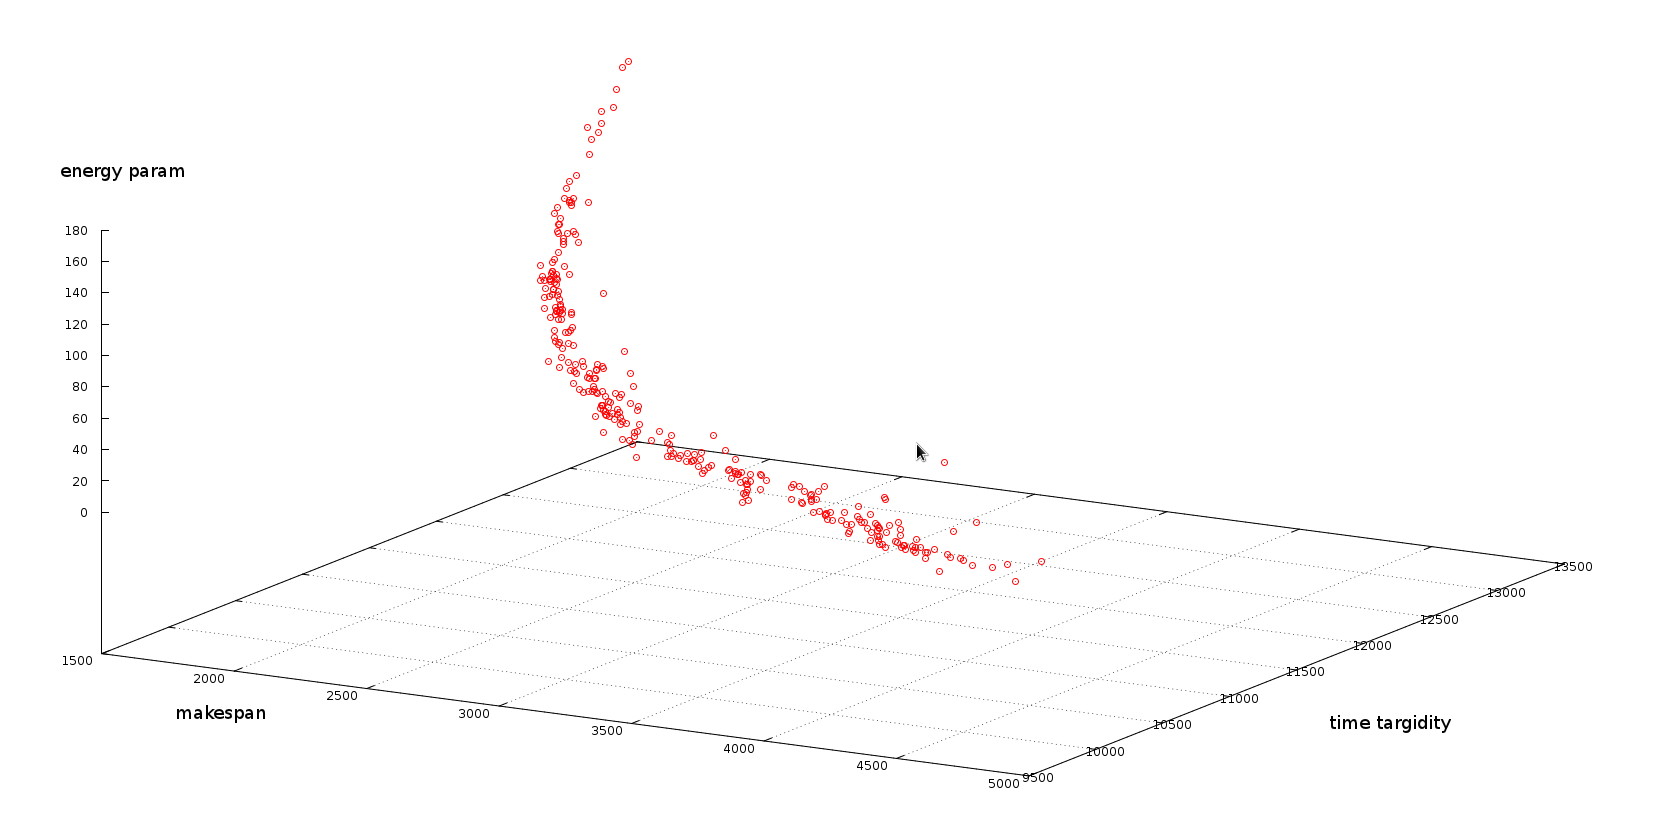
\includegraphics[width=1.0\columnwidth]{pareto}
    \caption{pareto front for makespan, time targidity and energy efficiency}
\label{pareto}
\end{figure}

\subsection{Experiment: Introducing job type constraint}
Now we introduce the job type constraint in our experimental analysis. Workload 3 and 4 referred in Table~\ref{datasets} have been used in this experiment. There are two type of jobs in the worload. On each workload we varied job percentage as 30\%-70\%, 50\%-50\%, 70\%-30\% to show the adaptiveness of our scheduler. 
A batch of 7000 jobs were taken which makes makespan of range $10^{7}$ to show the analysis in graph. Figure~\ref{jobtype1} shows uniform utilization among same type of resources inspite of the variance of job type percentage. One thing is further noticeable that analysis of section ~\ref{case2} still holds. Intel core i7 920 and Core i7-2600 performed equally well whereas Pentium 4 have disappointed again. \\
For choosing a scheduling strategy from first pareto front weighted sum technique on normalized objectives have been used. For the result shown in Figure~\ref{jobtype1} and ~\ref{jobtype2} equal weight was assigned on each objective.
\begin{figure}[h]
\centering
    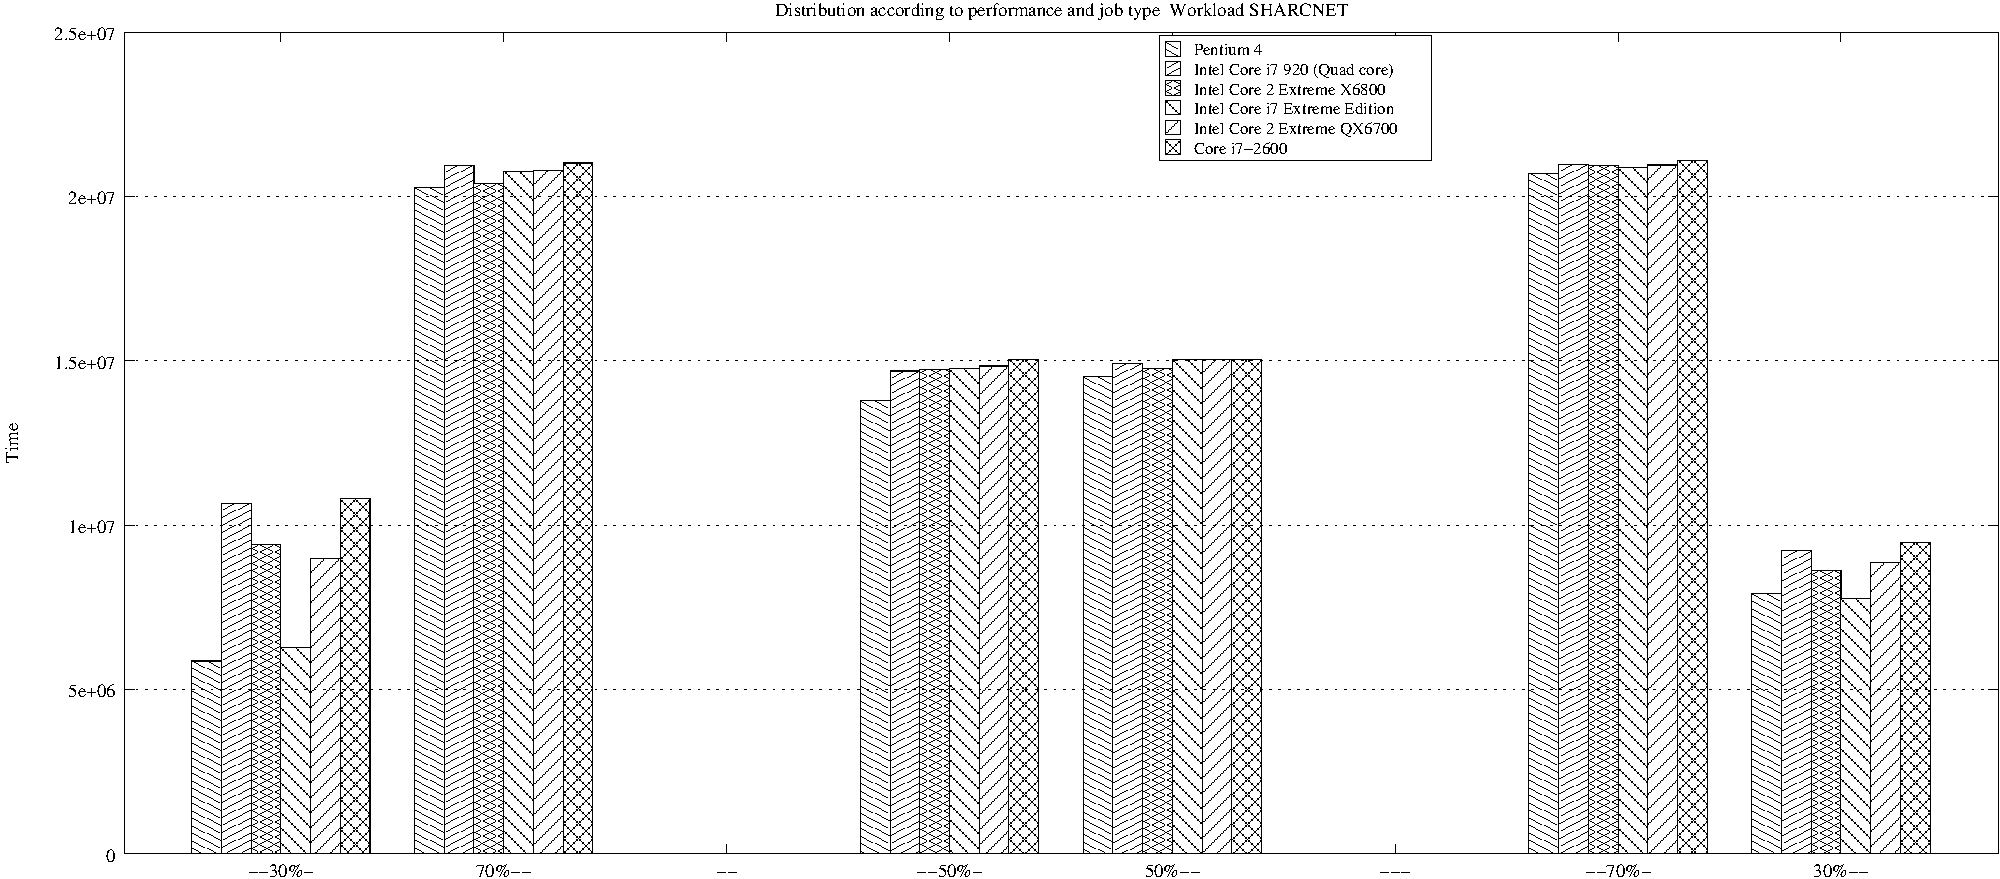
\includegraphics[width=1.0\columnwidth]{case3_SHARCNET}
    \caption{Performance under Job type constraint, SHARCNET Workload}
\label{jobtype1}
\end{figure}
\begin{figure}[h]
\centering
    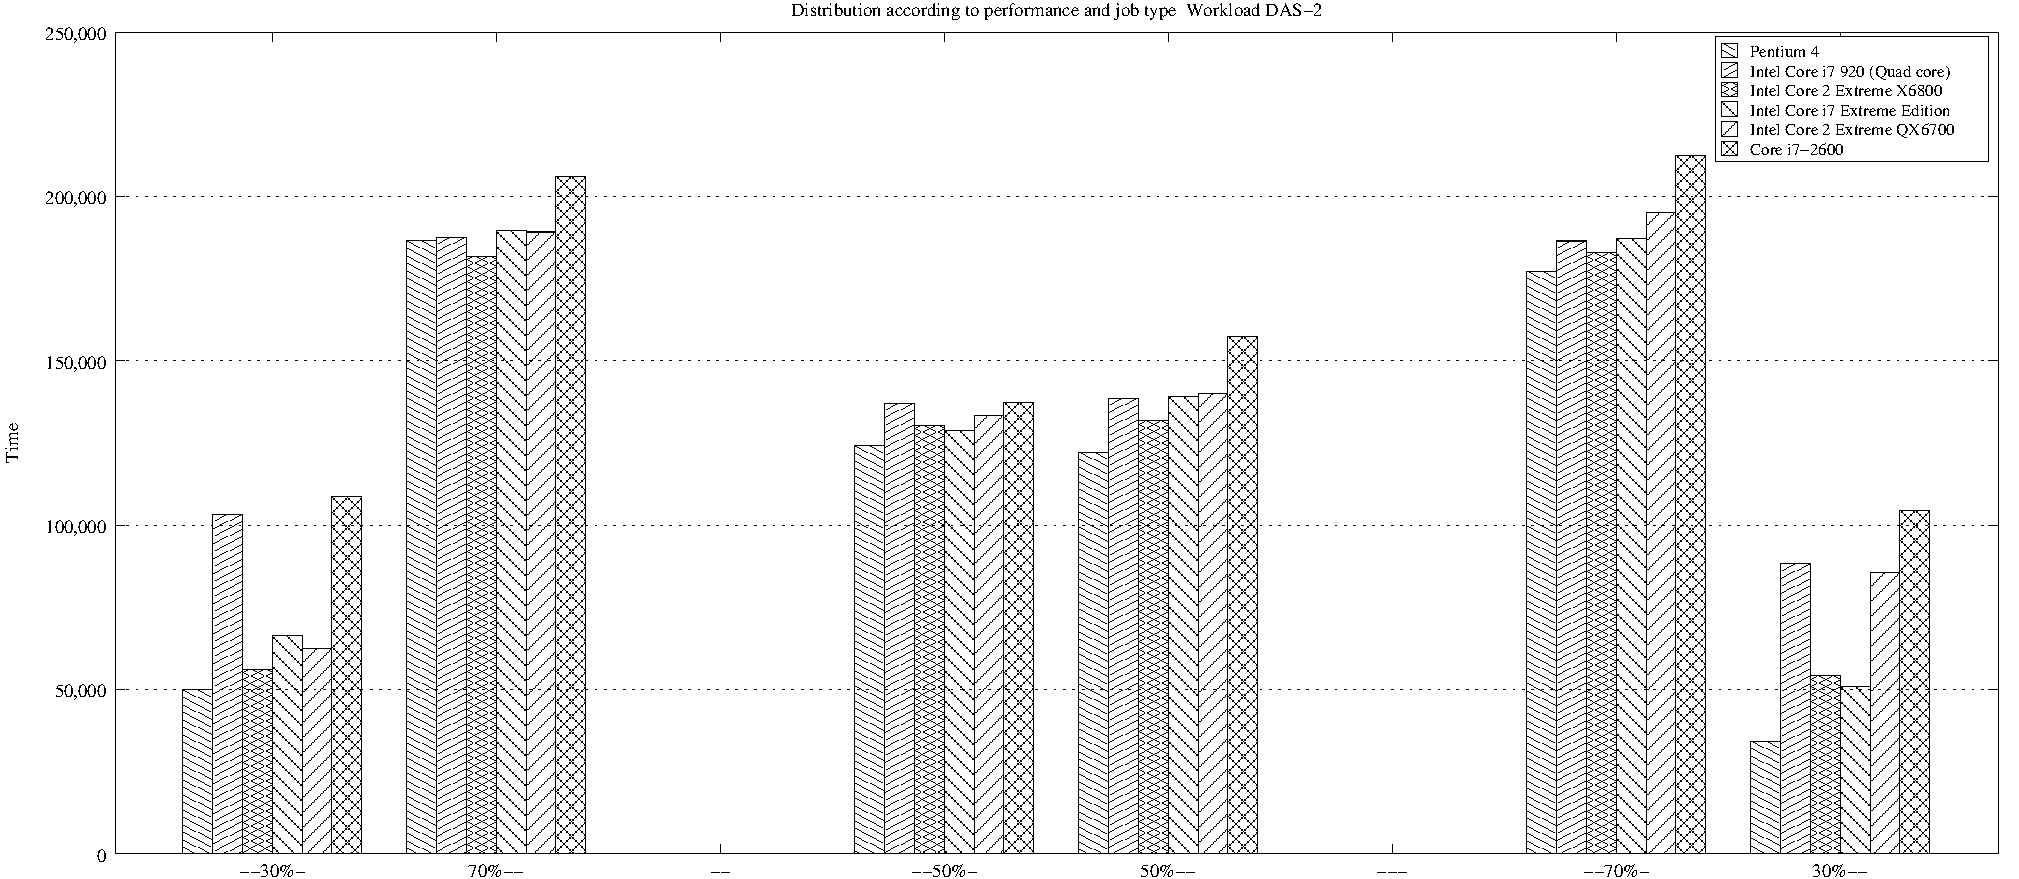
\includegraphics[width=1.0\columnwidth]{case3_DAS}
    \caption{Performance under Job type constraint, DAS-2 Workload}
\label{jobtype2}
\end{figure}

\subsection{Experiment: Introducing pricing model and precedence constraint}
\label{case4}
In this phase of experiment pricing parameter is incorporated in resource model. Experimented result shows how pricing model can change the utilization of resources. Workload 5 \&  6 have been used for this experiment having 50\% of job with predecessor dependencies referred in Table~\ref{datasets}. \\
Resources which are both low in performance and poor in energy efficiency is cheap in price, whereas high performance resource with less energy dissipation figure is preferred. Jobs having low job cost or high time limit can afford to run on these cheap resources whereas high priority jobs demanding high performance run on costly resources. Trade off among performance, time of execution and cost have allowed jobs to be scheduled on various resources uniformly. In table ~\ref{tab:sharccase4} \& ~\ref{tab:dascasse4}  it is observed that resources have adhered to the makespan and all have 98\%+ execution time. Utilization percentage shows actual uptime or running time of resources. This reveals that all resources have been utilized properly. Even resources like Pentium 4 have 95\% utilization on average.
\begin{framed}
{\small A question might arise in reader's mind ``Why resource utilization is not 100 percent?''. Jobs are having some precedence constraints; and a job scheduled on its compatible resource might take a little longer time to complete, forcing dependent jobs to wait on other idle resource. }
\end{framed}
In our experiment we have given equal weight to cost pricing, utilization of resources, time limit constraint and makespan. The grid administrator can configure the weight function to obtain required schedule strategy from first pareto front in search space like one given in figure ~\ref{pareto}.

\begin{table}[ht]
\caption{Resource Utilization after introduction of Job constraint and pricing model Workload 6 (SHARCNET)}
\scalebox{0.65}{
\begin{tabular}{|l|l|r|r|r|r|r|}
    \hline \hline
ID	&	Resource	&	Pricing model	&	Execution time	&	Makespan \%age	&	Actual utilized time	&	Utilization \%age	\\	\hline
1	&	Pentium 4	&	0.05	&	12048592.25	&	98.01	&	11813044.19	&	98.04	\\	\hline
2	&	Pentium 4	&	0.05	&	12163752.56	&	98.95	&	11300235.12	&	92.90	\\	\hline
3	&	Pentium 4	&	0.05	&	12164478.67	&	98.95	&	11686679.20	&	96.07	\\	\hline
4	&	Intel Core i7 920 (Quad core)	&	0.1	&	12046834.85	&	97.99	&	11272379.33	&	93.57	\\	\hline
5	&	Intel Core i7 920 (Quad core)	&	0.1	&	12047842.36	&	98.00	&	11749485.96	&	97.52	\\	\hline
6	&	Intel Core 2 Extreme X6800	&	0.09	&	12048727.00	&	98.01	&	11734951.47	&	97.39	\\	\hline
7	&	Intel Core 2 Extreme X6800	&	0.09	&	12160673.18	&	98.92	&	11776008.86	&	96.83	\\	\hline
8	&	Intel Core i7 Extreme Edition	&	0.15	&	12162928.27	&	98.94	&	11422999.16	&	93.91	\\	\hline
9	&	Intel Core i7 Extreme Edition	&	0.15	&	12160661.70	&	98.92	&	11777797.37	&	96.85	\\	\hline
10	&	Intel Core 2 Extreme QX6700	&	0.165	&	12160968.73	&	98.92	&	11864565.48	&	97.56	\\	\hline
11	&	Intel Core 2 Extreme QX6700	&	0.165	&	12156329.05	&	98.89	&	11976902.34	&	98.52	\\	\hline
12	&	Intel Core 2 Extreme QX6700	&	0.165	&	12160817.18	&	98.92	&	11727719.11	&	96.43	\\	\hline
13	&	Intel Core 2 Extreme QX6700	&	0.165	&	12160965.55	&	98.92	&	11931317.99	&	98.11	\\	\hline
14	&	Core i7-2600	&	0.18	&	12293364.46	&	100.00	&	11959913.00	&	97.28	\\	\hline
15	&	Core i7-2600	&	0.18	&	12161210.37	&	98.92	&	12059303.00	&	99.16	\\	\hline \hline
\end{tabular}
}
\label{tab:sharccase4}
\end{table}

\begin{table}[h]
\caption{Resource Utilization after introduction of Job constraint and pricing model Workload 5 (DAS-2)}
\centering
\scalebox{0.65}{
    \begin{tabular}{|l|l|r|r|r|r|r|}
    \hline \hline
ID	&	Resource	&	Pricing model	&	Execution time	&	Makespan \%age	&	Actual utilized time	&	Utilization \%age	\\	\hline
1	&	Pentium 4	&	0.05	&	307118.82	&	99.20	&	280545.30	&	91.34	\\	\hline
2	&	Pentium 4	&	0.05	&	301366.18	&	97.34	&	270360.92	&	89.71	\\	\hline
3	&	Pentium 4	&	0.05	&	300697.12	&	97.12	&	270477.22	&	89.95	\\	\hline
4	&	Intel Core i7 920 (Quad core)	&	0.1	&	307367.74	&	99.28	&	273357.18	&	88.93	\\	\hline
5	&	Intel Core i7 920 (Quad core)	&	0.1	&	307456.72	&	99.31	&	283748.63	&	92.28	\\	\hline
6	&	Intel Core 2 Extreme X6800	&	0.09	&	305703.06	&	98.74	&	269904.98	&	88.28	\\	\hline
7	&	Intel Core 2 Extreme X6800	&	0.09	&	305227.13	&	98.59	&	276089.83	&	90.45	\\	\hline
8	&	Intel Core i7 Extreme Edition	&	0.15	&	305428.16	&	98.65	&	288772.30	&	94.54	\\	\hline
9	&	Intel Core i7 Extreme Edition	&	0.15	&	303222.35	&	97.94	&	278433.59	&	91.82	\\	\hline
10	&	Intel Core 2 Extreme QX6700	&	0.165	&	309606.43	&	100.00	&	291890.84	&	94.27	\\	\hline
11	&	Intel Core 2 Extreme QX6700	&	0.165	&	309296.74	&	99.90	&	291225.75	&	94.15	\\	\hline
12	&	Intel Core 2 Extreme QX6700	&	0.165	&	305602.29	&	98.71	&	288181.42	&	94.29	\\	\hline
13	&	Intel Core 2 Extreme QX6700	&	0.165	&	303673.86	&	98.08	&	297436.40	&	97.94	\\	\hline
14	&	Core i7-2600	&	0.18	&	308464.86	&	99.63	&	303151.00	&	98.27	\\	\hline
15	&	Core i7-2600	&	0.18	&	308339.70	&	99.59	&	303203.00	&	98.33	\\	\hline \hline
\end{tabular}
}
\label{tab:dascasse4}
\end{table}
\subsection{Experiment with all constraints}
In this section we have incorporated all the constraints and evaluated our scheduler on workload 7 and 8 referred in Table~\ref{datasets}. Experiment is performed on 12 and 24 resources. For the sake of understanding equal number of resources for both type of jobs have been taken. \\
Results are given in Table ~\ref{case5das}, ~\ref{case5sha}, ~\ref{case5das24} and ~\ref{case5sha24}. There is no big difference with the result of Table~\ref{tab:dascasse4} and ~\ref{tab:sharccase4}. In this result, it is  observed that utilization percentage have dropped a little. Since jobs now have inter-resource type job dependencies utilization percentage drop is reasonable. Other performance parameter holds good. \\
An example of pareto front for this experiment is given in Figure~\ref{pareto3}  
\begin{figure}[h]
    \centering
    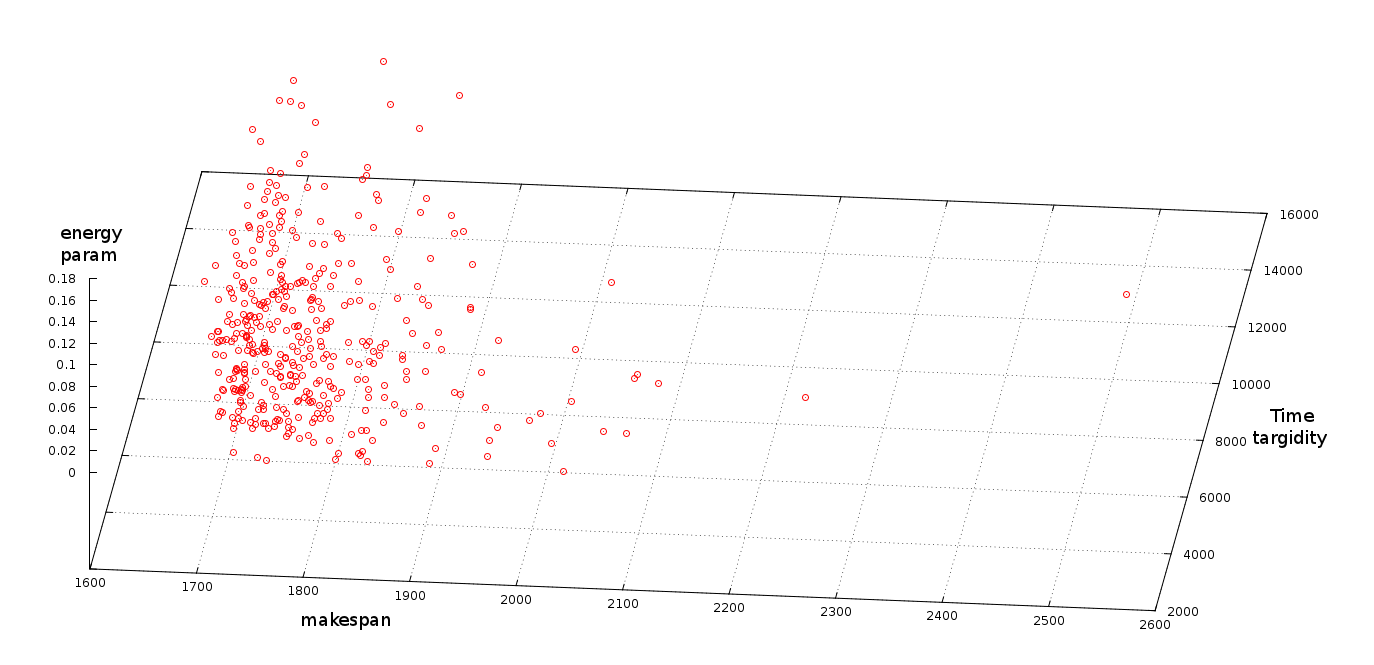
\includegraphics[width=1.0\columnwidth]{pareto3}
    \caption{Pareto front in experiment under all constraint}
    \label{pareto3}    
\end{figure}
    

\begin{table}[h]
\centering
\caption{Resource Utilization under all constraints on Workload DAS-2}
\scalebox{0.65}{
\begin{tabular}{|l|l|r|r|r|r|r|}
\hline \hline
ID	&	Resource	&	Pricing model	&	Execution time	&	Makespan \%age	&	Actual utilized time	&	Utilization \%age	\\	\hline
1	&	Pentium 4	&	0.05	&	388054.55346	&	95.31	&	337986.508894	&	87.10	\\	\hline
3	&	Intel Core i7 920 (Quad core)	&	0.1	&	390646.860537	&	95.95	&	362241.059321	&	92.72	\\	\hline
5	&	Intel Core 2 Extreme X6800	&	0.09	&	391917.860219	&	96.26	&	357671.610452	&	91.26	\\	\hline
7	&	Intel Core i7 Extreme Edition	&	0.15	&	389061.135613	&	95.56	&	367173.559685	&	94.37	\\	\hline
9	&	Intel Core 2 Extreme QX6700	&	0.165	&	389834.143125	&	95.75	&	368452.037427	&	94.51	\\	\hline
11	&	Core i7-2600	&	0.18	&	394967.616183	&	97.01	&	365376	&	92.50	\\	\hline
2	&	Pentium 4	&	0.05	&	407130.811479	&	100.00	&	362875.39219	&	89.12	\\	\hline
4	&	Intel Core i7 920 (Quad core)	&	0.1	&	406698.612175	&	99.89	&	343454.864029	&	84.44	\\	\hline
6	&	Intel Core 2 Extreme X6800	&	0.09	&	403146.303747	&	99.02	&	348012.012859	&	86.32	\\	\hline
8	&	Intel Core i7 Extreme Edition	&	0.15	&	402622.406754	&	98.89	&	378981.878416	&	94.12	\\	\hline
10	&	Intel Core 2 Extreme QX6700	&	0.165	&	405572.293961	&	99.62	&	385571.358202	&	95.06	\\	\hline
12	&	Core i7-2600	&	0.18	&	394268.616183	&	96.84	&	374894	&	95.08	\\	\hline \hline
\end{tabular}
}
\label{case5das}
\end{table}

\begin{table}[h]
\centering
\caption{Resource Utilization under all constraints on Workload SHARCNET }
\scalebox{0.65}{
    \begin{tabular}{|l|l|r|r|r|r|r|}
    \hline \hline
ID	&	Resource	&	Pricing model	&	Execution time	&	Makespan \%age	&	Actual utilized time	&	Utilization \%age	\\	\hline
1	&	Pentium 4	&	0.05	&	15856966.328786	&	99.65	&	14643863.906402	&	92.34	\\	\hline
3	&	Intel Core i7 920 (Quad core)	&	0.1	&	15777189.495383	&	99.14	&	14224208.443954	&	90.15	\\	\hline
5	&	Intel Core 2 Extreme X6800	&	0.09	&	15777954.142035	&	99.15	&	14347179.713218	&	90.93	\\	\hline
7	&	Intel Core i7 Extreme Edition	&	0.15	&	15853934.301256	&	99.63	&	14962167.332284	&	94.37	\\	\hline
9	&	Intel Core 2 Extreme QX6700	&	0.165	&	15855065.258749	&	99.63	&	14971170.083674	&	94.42	\\	\hline
11	&	Core i7-2600	&	0.18	&	15807884.835386	&	99.34	&	14039647	&	88.81	\\	\hline
2	&	Pentium 4	&	0.05	&	15855945.977623	&	99.64	&	15192585.514258	&	95.81	\\	\hline
4	&	Intel Core i7 920 (Quad core)	&	0.1	&	15856889.388767	&	99.65	&	15492772.72683	&	97.70	\\	\hline
6	&	Intel Core 2 Extreme X6800	&	0.09	&	15856577.788845	&	99.64	&	15509484.322644	&	97.81	\\	\hline
8	&	Intel Core i7 Extreme Edition	&	0.15	&	15808788.880171	&	99.34	&	15123906.518069	&	95.66	\\	\hline
10	&	Intel Core 2 Extreme QX6700	&	0.165	&	15913317.542563	&	100.00	&	15439774.23157	&	97.02	\\	\hline
12	&	Core i7-2600	&	0.18	&	15884947.971385	&	99.82	&	15685884	&	98.74	\\	\hline \hline
\end{tabular}
}
\label{case5sha}
\end{table}
\begin{table}[h]
\centering
\caption{Resource Utilization under all constraints on Workload SHARCNET }
\scalebox{0.65}{
    \begin{tabular}{|l|l|r|r|r|r|r|}
    \hline \hline
ID	&	Resource	&	Pricing model	&	Execution time	&	Makespan \%age	&	Actual utilized time	&	Utilization Percentage	\\	\hline
1	&	Pentium 4	&	0.05	&	8243698.72	&	99.49	&	7556234.165463	&	91.66	\\	\hline
2	&	Pentium 4	&	0.05	&	7275262.72	&	87.81	&	6253412.084217	&	85.95	\\	\hline
3	&	Intel Core i7 920 (Quad core)	&	0.1	&	7682671.48	&	92.72	&	6326204.11	&	82.34	\\	\hline
4	&	Intel Core i7 920 (Quad core)	&	0.1	&	8233315.82	&	99.37	&	7351339.16	&	89.28	\\	\hline
5	&	Intel Core 2 Extreme X6800	&	0.09	&	8117606.74	&	97.97	&	7269743.03	&	89.55	\\	\hline
6	&	Intel Core 2 Extreme X6800	&	0.09	&	8118002.88	&	97.98	&	7072373.18	&	87.11	\\	\hline
7	&	Intel Core i7 Extreme Edition	&	0.15	&	8117468.76	&	97.97	&	7183725.78	&	88.49	\\	\hline
8	&	Intel Core i7 Extreme Edition	&	0.15	&	8244584.64	&	99.50	&	7426916.89	&	90.08	\\	\hline
9	&	Intel Core 2 Extreme QX6700	&	0.165	&	8117904.66	&	97.98	&	7220275.87	&	88.94	\\	\hline
10	&	Intel Core 2 Extreme QX6700	&	0.165	&	8119335.22	&	97.99	&	7202661.19	&	88.70	\\	\hline
11	&	Core i7-2600	&	0.18	&	8229761.81	&	99.33	&	7763631	&	94.33	\\	\hline
12	&	Core i7-2600	&	0.18	&	8244728.91	&	99.51	&	7615311	&	92.36	\\	\hline
13	&	Pentium 4	&	0.05	&	8119374.38	&	97.99	&	7906705.979229	&	97.38	\\	\hline
14	&	Pentium 4	&	0.05	&	8231574.39	&	99.35	&	7705017.3826	&	93.60	\\	\hline
15	&	Intel Core i7 920 (Quad core)	&	0.1	&	8229150.06	&	99.32	&	7628743.04	&	92.70	\\	\hline
16	&	Intel Core i7 920 (Quad core)	&	0.1	&	8117134.83	&	97.97	&	7339766.91	&	90.42	\\	\hline
17	&	Intel Core 2 Extreme X6800	&	0.09	&	8244402.12	&	99.50	&	7126312.76	&	86.43	\\	\hline
18	&	Intel Core 2 Extreme X6800	&	0.09	&	8120187.28	&	98.00	&	7600934.79	&	93.60	\\	\hline
19	&	Intel Core i7 Extreme Edition	&	0.15	&	8285650.01	&	100.00	&	8151742.16	&	98.38	\\	\hline
20	&	Intel Core i7 Extreme Edition	&	0.15	&	8230477.53	&	99.33	&	7746832.68	&	94.12	\\	\hline
21	&	Intel Core 2 Extreme QX6700	&	0.165	&	8232608.55	&	99.36	&	7776374.29	&	94.45	\\	\hline
22	&	Intel Core 2 Extreme QX6700	&	0.165	&	8230191.41	&	99.33	&	7517359.04	&	91.33	\\	\hline
23	&	Core i7-2600	&	0.18	&	8244461.91	&	99.50	&	7950420	&	96.43	\\	\hline
24	&	Core i7-2600	&	0.18	&	8244329.91	&	99.50	&	7745014	&	93.94	\\	\hline
\end{tabular}
}
\label{case5sha24}
\end{table}

\begin{table}[!h]
\centering
\caption{Resource Utilization under all constraints on Workload DAS-2 }
\scalebox{0.65}{
    \begin{tabular}{|l|l|r|r|r|r|r|}
    \hline \hline
ID	&	Resource	&	Pricing model	&	Execution time	&	Makespan \%age	&	Actual utilized time	&	Utilization Percentage	\\	\hline
1	&	Pentium 4	&	0.05	&	219982.24	&	97.21	&	163440.56	&	74.29	\\	\hline
2	&	Pentium 4	&	0.05	&	219542.01	&	97.02	&	174237.89	&	79.36	\\	\hline
3	&	Intel Core i7 920 (Quad core)	&	0.1	&	219052.01	&	96.80	&	165654.30	&	75.62	\\	\hline
4	&	Intel Core i7 920 (Quad core)	&	0.1	&	216803.93	&	95.81	&	184625.00	&	85.15	\\	\hline
5	&	Intel Core 2 Extreme X6800	&	0.09	&	219223.62	&	96.88	&	182191.65	&	83.10	\\	\hline
6	&	Intel Core 2 Extreme X6800	&	0.09	&	219492.39	&	97.00	&	174748.10	&	79.61	\\	\hline
7	&	Intel Core i7 Extreme Edition	&	0.15	&	219025.20	&	96.79	&	181810.38	&	83.00	\\	\hline
8	&	Intel Core i7 Extreme Edition	&	0.15	&	220180.92	&	97.30	&	188177.47	&	85.46	\\	\hline
9	&	Intel Core 2 Extreme QX6700	&	0.165	&	224356.86	&	99.15	&	177056.99	&	78.91	\\	\hline
10	&	Intel Core 2 Extreme QX6700	&	0.165	&	195262.07	&	86.29	&	171776.61	&	87.97	\\	\hline
11	&	Core i7-2600	&	0.18	&	219419.10	&	96.97	&	190443	&	86.79	\\	\hline
12	&	Core i7-2600	&	0.18	&	218241.87	&	96.45	&	199849	&	91.57	\\	\hline
13	&	Pentium 4	&	0.05	&	218245.15	&	96.45	&	193682.53	&	88.74	\\	\hline
14	&	Pentium 4	&	0.05	&	221455.49	&	97.87	&	179685.28	&	81.13	\\	\hline
15	&	Intel Core i7 920 (Quad core)	&	0.1	&	220399.63	&	97.40	&	173087.60	&	78.53	\\	\hline
16	&	Intel Core i7 920 (Quad core)	&	0.1	&	223197.97	&	98.64	&	184545.05	&	82.68	\\	\hline
17	&	Intel Core 2 Extreme X6800	&	0.09	&	223858.93	&	98.93	&	187562.65	&	83.78	\\	\hline
18	&	Intel Core 2 Extreme X6800	&	0.09	&	221743.64	&	97.99	&	189665.95	&	85.53	\\	\hline
19	&	Intel Core i7 Extreme Edition	&	0.15	&	225453.79	&	99.63	&	164904.97	&	73.14	\\	\hline
20	&	Intel Core i7 Extreme Edition	&	0.15	&	226286.04	&	100.00	&	178501.31	&	78.88	\\	\hline
21	&	Intel Core 2 Extreme QX6700	&	0.165	&	224749.06	&	99.32	&	188318.89	&	83.79	\\	\hline
22	&	Intel Core 2 Extreme QX6700	&	0.165	&	225663.04	&	99.72	&	184520.37	&	81.76	\\	\hline
23	&	Core i7-2600	&	0.18	&	222377.53	&	98.27	&	196349	&	88.29	\\	\hline
24	&	Core i7-2600	&	0.18	&	223615.40	&	98.82	&	201232	&	89.99	\\	\hline
\end{tabular}
}
\label{case5das24}
\end{table}


\section{Conclusion}
The main motive of this work is to provide a flexible scheduler keeping multiple objectives into consideration. The scheduler module yields best scheduling strategies on various parameters in a pareto front. This is upto grid administrator and dynamic grid environment to choose a scheduling strategy of its choice. For experimentation purpose we have put equal weights on each objective for choosing best scheduling strategy. \\
Our results clearly shows that our scheduler produces optimized schedule on multi-objective optimization environment. The scheduler is scalable with resources and can process an infinite queue of jobs. The scheduler responded well with the change of constraints and behaviour of grid and job model. All resources have adhered to the makespan, and utilization rate is also high inspite of precedence constraint. It is difficult to display minimization of cost and time targidity parameter in graph or table. However a live demo of search space graph with schedules/chromosomes on successive iteration of genetic algorithm can verify its authenticity (Refer to User's Manual in Appendix~\ref{userman}). 
\\
